\documentclass[11pt,a4paper]{article}
\usepackage{amsmath,amssymb,graphicx,geometry,booktabs,hyperref,longtable}
\usepackage{setspace}
\onehalfspacing
\emergencystretch=1.5em
\geometry{margin=1in}

\title{\textbf{Does Mandatory ESG Disclosure Change Corporate Hedging?\\
Theory, and Evidence from Korea's Staggered Disclosure Mandates}}
\author{\textbf{Jihong Park} \\ Pusan National University}
\date{July 2026}

\begin{document}

\maketitle

\begin{abstract}
Does mandatory ESG disclosure change how firms hedge? I model a firm that jointly chooses hedge ratios and disclosure intensity, where disclosure operates only through the price the firm attaches to residual risk. The model yields closed-form hedge ratios and signed comparative statics: stricter regimes raise hedging unconditionally, whereas the disclosure response depends on whether the firm's own distress-cost motive outweighs the marginal regulatory penalty. I test the model on Korea's two ESG-disclosure mandates with realized adoption -- the corporate-governance report, phased in by asset tier over 2019--2024, and the environmental-information requirement binding large issuers from 2022 -- using a 380-firm, 3{,}420 firm-year panel of KOSPI issuers built from OpenDART filings, with every annual report parsed for hedge-accounting designation and derivative usage. Group-time ATT estimates are precise nulls on both real margins for both mandates, robust to three comparison-set rules, with placebo tests indistinguishable from zero; confidence intervals exclude effects beyond roughly six percentage points. The nulls identify the disclosure--hedging channel as risk-specific: mandates that leave the firm's market-risk exposure unquantified -- even ones compelling quantitative environmental data -- leave its hedging incentive unchanged. The climate mandate, which compels quantification of the exposure itself, is the model's standing prediction and is testable on this pipeline as its phase-ins complete.
\end{abstract}

\noindent\textbf{Keywords:} ESG disclosure; corporate hedging; hedge accounting; IFRS 9; difference-in-differences; staggered adoption; derivatives; climate risk; Korea; OpenDART.\\
\textbf{JEL codes:} G32 (financing policy; risk management), G38 (government policy and regulation), M41 (accounting), M48 (government policy and regulation), Q54 (climate), C23 (panel data models).

\tableofcontents
\newpage

% =============================================================================
\section{Introduction}
\label{sec:intro}

The three companion papers in this program hold one economic position fixed -- a Korean crude-oil importer's joint exposure to the WTI price of its physical barrels and the USD/KRW rate at which the dollar liability converts to won -- and interrogate it from three angles: the static allocation of a fixed premium budget across the two legs (Park, 2026a), the path-by-path performance of a dynamic delta hedge of a quanto knock-out written on the same exposure (Park, 2026c), and the IFRS~9 hedge-accounting treatment of the resulting relationship (Park, 2026b). All three take the \emph{decision to hedge}, and its intensity, as a primitive. This paper asks what sets that primitive. Specifically: does a change in the firm's \emph{disclosure} environment -- the arrival of a mandatory ESG and climate-risk reporting regime -- change how much of its commodity and currency risk a firm hedges, whether it elects hedge accounting, and how efficiently it converts hedging spend into volatility reduction?

The question is neither the familiar ``does ESG raise firm value'' correlation nor a reporting-quality exercise. It is a risk-management question with a specific mechanism. A disclosure mandate does two things at once to a firm carrying real financial and climate exposure. First, it raises the marginal cost of \emph{leaving risk unhedged}: once a firm must quantify and publish its climate-related financial exposures (KSSB/ISSB S2), residual exposure becomes visible to investors, lenders, and supervisors, and the penalty for carrying it -- through cost of capital, covenant scrutiny, and reputational channels -- rises. Second, disclosure is itself costly, and the firm chooses how much of it to produce. The firm therefore solves a joint problem in three instruments: how much financial risk to hedge, how much climate risk to hedge, and how much to disclose. The central economic content is that these instruments are coupled -- disclosure intensity shifts the shadow price of residual risk, which shifts the optimal hedge ratios -- and that the coupling has a sign the data can be asked to confirm.

Korea is an unusually clean laboratory for this question, because it has legislated a sequence of ESG-disclosure mandates that differ in exactly the dimension the model prices: how directly the required disclosure quantifies the firm's risk exposure. The mandatory corporate-governance report (phased in by asset tier: 2019, 2022, 2024) obliges disclosure about board structure and control -- the G pillar -- without touching exposure. The environmental-information disclosure requirement (from 2022, for listed firms with assets above KRW 2 trillion) obliges quantitative reporting of emissions and resource use -- exposure-adjacent, but not market-risk exposure. The KSSB's ISSB-aligned climate standards (mirroring IFRS~S1/S2), whose phase-ins are pending, will oblige quantification of climate-related \emph{financial} exposure itself. Each mandate phases in by size tier, generating the staggered treatment structure that modern difference-in-differences estimation exploits, with not-yet-covered firms as controls. Korea also has a centralized, machine-readable filing system -- the Financial Supervisory Service's OpenDART -- that makes the required firm-level panel constructible from primary filings.

This paper makes three moves, matching the structure of its companions. First (Section~\ref{sec:model}), it writes down the firm's joint hedging-and-disclosure problem and solves it: the interior optimum in the two hedge ratios is a closed-form linear-system solution driven by the risk covariance matrix and the premium vector, scaled by a disclosure-dependent effective risk price $\Lambda(d)=\phi+\lambda e^{-kd}$; the disclosure choice is the solution of a scalar first-order condition balancing quadratic disclosure cost against exponential penalty relief. From this the paper \emph{derives}, rather than asserts, the comparative statics that the empirics then test -- most importantly $\partial h_f/\partial\lambda>0$ (a tougher penalty regime unambiguously raises hedging), $\partial h_f/\partial a>0$ (when disclosure is expensive, firms substitute toward hedging), and a closed-form sign for the correlation sensitivity $\partial h_f/\partial\rho$. The disclosure response is subtler and the derivation is careful about it: because hedging and disclosure are substitutes in the penalty channel, $\partial d^\star/\partial\lambda$ carries the sign of $\phi-\lambda e^{-kd^\star}$ -- disclosure rises with stringency only when the firm's own distress-cost motive dominates the marginal regulatory penalty -- so ``tougher regime, more disclosure'' is a conditional, not an unconditional, prediction. Second (Sections~\ref{sec:hypotheses}--\ref{sec:design}), it converts the comparative statics into formal hypotheses and an identification strategy: a heterogeneity-robust staggered DiD with an event-study parallel-trends test, backed by synthetic-control, triple-difference, and instrumental-variable alternatives. Third (Section~\ref{sec:data}), it specifies the Korean data pipeline in full -- sources, XBRL tags, proxy definitions, winsorization, and missing-data rules -- and executes its structured front live against the OpenDART API (Section~\ref{sec:pilot}), retrieving a real pilot sample and parsing the derivative notes -- which shows the hedge-accounting designation reliably extractable but the numeric derivative tables heterogeneous across firms, locating the true remaining obstacle rather than leaving the pipeline hypothetical.

This paper pairs a closed-form theory with an executed empirical test. The design was written for the KSSB climate mandate, which has no realized post-period yet; Section~\ref{sec:executed} therefore runs the design on Korea's two realized ESG-disclosure mandates -- the staggered governance report (2019/2022/2024 by asset tier) and the environmental-information requirement (2022, assets $\ge$2tn) -- on a 380-firm, 3{,}420 firm-year panel built from OpenDART filings. Both mandates produce precise nulls on every real hedging margin, robust across three comparison-set rules, with placebo estimates indistinguishable from zero; a placebo test during construction also identified an encoding artifact in older filings that would otherwise have masqueraded as a positive effect. Read through the model, the nulls identify the penalty channel as risk-specific: neither mandate forces quantification of market-risk exposure, so neither moves the hedging-relevant residual-risk price, and the climate mandate -- which does force it -- becomes the standing falsifiable test. A companion engine (Section~\ref{sec:numerics}) separately certifies the solver against an independent optimizer and shows the estimators recover known effects on model-generated panels; Section~\ref{sec:robust} builds the design around its principal identification threats -- endogenous timing, measurement, staggered-adoption bias, and functional-form dependence.

% =============================================================================
\section{Literature Review}
\label{sec:lit}

This paper sits at the intersection of five literatures: the theory of corporate hedging, the empirics of derivative usage and firm value, hedge accounting under IFRS, the economics of mandatory ESG and climate disclosure, and the econometrics of staggered policy adoption. Table~\ref{tab:litmap} maps the indispensable works in each; the text then states precisely how the present design differs.

\paragraph{Corporate hedging theory.} The rationale for costly hedging by value-maximizing firms is the foundation the disclosure question builds on. Smith and Stulz (1985) derive hedging from convexity in taxes, distress costs, and managerial risk aversion; Froot, Scharfstein, and Stein (1993) reframe hedging as the protection of internal funds for investment when external finance is costly, which is the friction that makes a residual-risk penalty economically real rather than a modeling device; and Stulz (1996) rationalizes \emph{selective, partial} hedging -- exactly the interior $h<1$ the present model produces. These papers explain \emph{why} $\lambda>0$; none of them lets the shadow price of residual risk be moved by a disclosure choice, which is this paper's mechanism. Adler and Dumas (1984) supply the definition of currency exposure the financial leg uses, and Anderson and Danthine (1981) and Ederington (1979) the cross-hedging and minimum-variance-ratio apparatus that the covariance-matrix solution of Section~\ref{sec:model} specializes.

\paragraph{Derivative usage and firm value.} The empirical hedging literature establishes both the determinants and the measurement of corporate derivative use, and is the direct methodological ancestor of the design here. Nance, Smith, and Smithson (1993) and G\'eczy, Minton, and Schrand (1997) identify the firm characteristics -- size, growth options, financial constraint, foreign exposure -- that predict derivative use and that this design carries as controls $X_{it}$. Tufano (1996) and Jin and Jorion (2006) study commodity producers, the mirror image of the importer position of the companion papers. Allayannis and Weston (2001), Graham and Rogers (2002), Guay and Kothari (2003), and Bartram, Brown, and Conrad (2011) develop the notional- and sensitivity-based measures of hedging intensity and its value and risk consequences that the proxies of Section~\ref{sec:data} adopt. What none of these studies has is an exogenous shifter of the \emph{disclosure} environment; they treat hedging as a function of firm fundamentals, whereas this design uses a disclosure mandate as a quasi-experimental shock to the hedging decision itself.

\paragraph{Hedge accounting under IFRS.} Glaum and Kl\"ocker (2011) document that hedge-accounting eligibility feeds back into firms' real hedging choices -- ``the tail wags the dog'' -- which is why the hedge-accounting-adoption dummy is a dependent variable here and not merely a control. Panaretou, Shackleton, and Taylor (2013) study the information effects of IFRS hedge-accounting disclosure in the UK. The companion paper (Park, 2026b) supplies the path-wise IFRS~9 cash-flow-hedge accounting engine whose designation architecture -- combined quanto versus split risk-component -- this paper treats as one of the firm's response margins to disclosure. IAS~39 and IFRS~9 (IASB, 2014) define the effectiveness and cost-of-hedging mechanics.

\paragraph{Mandatory ESG and climate disclosure.} The disclosure-economics literature is where the identifying variation lives. Christensen, Hail, and Leuz (2021) survey, on economic-analysis grounds, what mandatory CSR and sustainability reporting can and cannot be expected to do, and caution that real-decision effects (as opposed to reporting effects) are the harder object to identify -- a caution this design takes seriously by making a \emph{real} choice (hedging) the outcome. Chen, Hung, and Wang (2018) and Downar et al.\ (2021) exploit mandated CSR and carbon disclosure to identify real effects; Grewal, Riedl, and Serafeim (2019) study market reactions to the EU nonfinancial-disclosure mandate; Krueger, Sautner, Tang, and Zhang (2024) provide cross-country evidence on the effects of mandatory ESG disclosure. On the climate-risk side, Krueger, Sautner, and Starks (2020) and Ilhan, Krueger, Sautner, and Starks (2023) document that institutional investors price and demand climate-risk disclosure; Bolton and Kacperczyk (2021) document a carbon premium; and Engle, Giglio, Kelly, Lee, and Stroebel (2020) and Hong, Li, and Xu (2019) develop the climate-risk-hedging constructs the climate-hedge ratio $h_c$ operationalizes. What is missing across this literature is a structural link from the disclosure mandate to the \emph{derivatives and hedge-accounting} response specifically; existing work studies emissions, investment, or cost of capital, not the hedge ratio.

\paragraph{Econometrics of staggered adoption.} Because Korea's mandate phases in by tier, the design must use the modern DiD toolkit. Bertrand, Duflo, and Mullainathan (2004) establish the inference problem in DiD with serial correlation; Goodman-Bacon (2021) shows how two-way fixed-effects DiD decomposes -- and can be biased -- under staggered timing; Callaway and Sant'Anna (2021), Sun and Abraham (2021), and de Chaisemartin and D'Haultf\oe uille (2020) supply the heterogeneity-robust group-time estimators this paper uses in place of naive TWFE; and Abadie, Diamond, and Hainmueller (2010) supply the synthetic-control alternative for the largest treated firms, which have the thinnest comparison sets.

\begin{table}[h]
\centering
\small
\begin{tabular}{p{3.0cm} p{4.4cm} p{3.0cm} p{3.6cm}}
\toprule
Category & Representative works & Method / data & How this paper differs \\
\midrule
Hedging theory & Smith--Stulz (1985); Froot--Scharfstein--Stein (1993); Stulz (1996) & Analytical models of costly hedging & Lets the residual-risk price be endogenous to a disclosure choice \\
Cross-hedging & Anderson--Danthine (1981); Ederington (1979); Adler--Dumas (1984) & Minimum-variance ratios & Two coupled exposures with a disclosure-scaled risk price \\
Derivative use \& value & Nance et al.\ (1993); G\'eczy et al.\ (1997); Allayannis--Weston (2001); Bartram et al.\ (2011); Jin--Jorion (2006) & Cross-sectional / panel; notional \& sensitivity proxies & Uses a disclosure mandate as a quasi-experiment on hedging \\
Hedge accounting & Glaum--Kl\"ocker (2011); Panaretou et al.\ (2013); IASB (2014) & Survey / archival; IFRS~9 mechanics & Hedge-accounting adoption as an outcome of disclosure regulation \\
ESG / climate disclosure & Christensen et al.\ (2021); Chen et al.\ (2018); Downar et al.\ (2021); Krueger et al.\ (2020, 2024); Ilhan et al.\ (2023) & Mandate-based DiD; investor surveys & Links the mandate to derivatives \& hedge accounting, not emissions \\
Climate-risk hedging & Engle et al.\ (2020); Hong et al.\ (2019); Bolton--Kacperczyk (2021) & Return-based hedge portfolios & Operationalizes a firm-level climate-hedge ratio $h_c$ \\
Staggered DiD & Goodman-Bacon (2021); Callaway--Sant'Anna (2021); Sun--Abraham (2021); de Chaisemartin--D'Haultf.\ (2020); Abadie et al.\ (2010) & Group-time ATT; synthetic control & Applies heterogeneity-robust estimators to a phased Korean mandate \\
\bottomrule
\end{tabular}
\caption{Literature map. Indispensable works are those defining the residual-risk-price mechanism (Froot--Scharfstein--Stein; Stulz), the hedging-measurement apparatus (G\'eczy et al.; Bartram et al.), the mandate-as-quasi-experiment template (Christensen et al.; Downar et al.), and the heterogeneity-robust estimator (Callaway--Sant'Anna; Sun--Abraham). The climate-return-hedging works (Engle et al.; Hong et al.) are supporting rather than indispensable.}
\label{tab:litmap}
\end{table}

% =============================================================================
\section{A Model of Joint Hedging and Disclosure Choice}
\label{sec:model}

\subsection{Setup and decision variables}
\label{sec:setup}

A firm carries two zero-mean risk exposures over one period: a financial exposure (the commodity-and-currency risk of the companion papers, collapsed for tractability into one factor with volatility $\sigma_f$) and a climate-related financial exposure with volatility $\sigma_c$, correlated at $\rho$. The firm chooses three instruments:
\begin{equation}
h_f\in[0,1]\quad(\text{financial hedge ratio}),\qquad h_c\in[0,1]\quad(\text{climate hedge ratio}),\qquad d\ge 0\quad(\text{disclosure intensity}).
\end{equation}
Hedging fraction $h_f$ removes that fraction of the financial exposure's standard deviation and $h_c$ that of the climate exposure; the \emph{unhedged} fractions are $1-h_f$ and $1-h_c$. Writing the risk covariance matrix
\begin{equation}
\Sigma=\begin{pmatrix}\sigma_f^2 & \rho\,\sigma_f\sigma_c\\[2pt] \rho\,\sigma_f\sigma_c & \sigma_c^2\end{pmatrix},\qquad
u\equiv 1-h_f,\quad v\equiv 1-h_c,\quad \mathbf{u}\equiv(u,v)^\top,
\end{equation}
the residual exposure (variance of the unhedged portfolio) is the quadratic form
\begin{equation}
R(h_f,h_c)\;=\;\mathbf{u}^\top\Sigma\,\mathbf{u}\;=\;(1-h_f)^2\sigma_f^2+(1-h_c)^2\sigma_c^2+2\rho\,\sigma_f\sigma_c(1-h_f)(1-h_c).
\label{eq:R}
\end{equation}

\paragraph{A remark on timing.}
The model is written as one period, but the two choices do not live on the same clock: disclosure intensity is an infrastructure stock -- reporting systems, controls, assurance relationships -- while hedge ratios are flow decisions reset at each derivative roll. The one-period objective should be read as the per-period value of the corresponding two-stage problem in which $d$ is committed first at amortized cost and the hedges follow each period given $d$. Because the equilibrium below solves recursively -- hedges in closed form given $\Lambda(d)$, then $d^\star$ from a scalar fixed point -- the static solution coincides with the stationary policy of that two-timescale problem, and nothing in the comparative statics depends on the compression. What the reduction genuinely omits is the \emph{transition}: a mandate arriving mid-stream forces adjustment of the disclosure stock at a pace the model does not price. That omission has an econometric counterpart rather than a fix -- the event-study coefficients of Section~\ref{sec:design} trace the transition path to the new stationary policy, and should not be read as instantaneous jumps between steady states.

\subsection{Costs and the firm's problem}
\label{sec:problem}

Total cost has four components. Hedging carries a linear premium in each leg,
\begin{equation}
C_H=p_f\,h_f+p_c\,h_c,
\end{equation}
with $p_f,p_c>0$ the per-unit premia (the option-budget objects priced in Park, 2026a). Disclosure is convex,
\begin{equation}
C_D=a\,d^2,\qquad a>0,
\end{equation}
capturing the increasing marginal cost of producing and assuring incremental ESG/climate disclosure. The coefficient $a$ is firm-specific in everything that follows, and no claim is made that it is exogenous in the cross-section -- the firm that runs a derivatives desk cheaply plausibly also staffs a reporting function cheaply, so $a$ and risk-management capability are likely entangled. The equilibrium requires only that $a$ be a parameter of the firm's problem; what the \emph{empirical} use of the $a$-comparative-static requires is the sharper condition that $a$ be predetermined with respect to mandate timing, and the numerical engine (Appendix~\ref{sec:appendix}) quantifies how a capability confound of exactly this form biases the interaction test -- the reason H(sub) is carried as exploratory rather than load-bearing. Residual risk carries a baseline economic cost -- the distress- and financing-friction cost of Froot--Scharfstein--Stein --
\begin{equation}
C_R=\phi\,R(h_f,h_c),\qquad \phi\ge 0,
\end{equation}
and, on top of it, a \emph{disclosure-contingent regulatory penalty}
\begin{equation}
P=\lambda\,R(h_f,h_c)\,e^{-kd},\qquad \lambda>0,\ k>0.
\label{eq:penalty}
\end{equation}
The penalty is the mechanism. Its magnitude scales with residual exposure $R$ (a firm that carries more unhedged risk is penalized more once that risk is visible), with the regime's stringency $\lambda$ (the regulator's dial), and it is \emph{attenuated} by disclosure: $e^{-kd}$ falls from $1$ toward $0$ as the firm discloses more, because disclosure converts opaque exposure into quantified, investor-legible exposure that the firm can then be seen to be managing, softening the cost-of-capital and reputational bite of a given $R$.\footnote{The exponential form is the natural one-parameter attenuation: $P>0$ for all finite $d$, $\partial P/\partial d<0$, and $P\to 0$ only in the limit of unbounded disclosure, so disclosure never fully substitutes for hedging. It also keeps the disclosure first-order condition analytically closed. A power-law attenuation $R(1+kd)^{-1}$ yields the same comparative-statics signs.}

\paragraph{A screening micro-foundation for the exponential.}
The functional form need not be defended on tractability alone. Suppose the penalty is levied on residual exposure only while that exposure remains \emph{illegible} to the pricing audience -- the regulator, lenders, rating agencies -- and that each unit of disclosure intensity generates independent verifiable signals that resolve the firm's opacity at constant hazard $k$, the Poisson-verification benchmark of the inspection and auditing literature (Townsend, 1979; Dye, 1986). The probability that the exposure is still unpriced after $d$ units of disclosure is then $e^{-kd}$, and the \emph{expected} penalty is exactly $\lambda R\,e^{-kd}$: equation~\eqref{eq:penalty} is the reduced form of a verification technology, and $k$ is the informativeness of a unit of disclosure -- assurance quality, standardization, machine-readability -- rather than a free curvature parameter. Two consequences follow. First, the mechanism this foundation pins down is information resolution; a cost-of-capital repricing story generates the same reduced form, and the two are observationally equivalent within it -- the model prices the friction without adjudicating its channel (Section~\ref{sec:discussion} returns to this). Second, $k$ acquires an empirical counterpart: disclosure that is assured or filed under a standardized taxonomy should carry a higher $k$ than narrative reporting, a cross-sectional restriction the design can exploit when assurance data become available.

Collecting terms, and defining the \emph{effective marginal price of residual risk}
\begin{equation}
\boxed{\ \Lambda(d)\;\equiv\;\phi+\lambda e^{-kd}\ }\qquad(\Lambda>0,\ \Lambda'(d)=-k\lambda e^{-kd}<0),
\label{eq:Lambda}
\end{equation}
the firm's problem is
\begin{equation}
\min_{h_f\in[0,1],\,h_c\in[0,1],\,d\ge0}\ \Pi(h_f,h_c,d)\;=\;p_f h_f+p_c h_c+a d^2+\Lambda(d)\,R(h_f,h_c).
\label{eq:objective}
\end{equation}
Equation~\eqref{eq:objective} is the paper's economic core: disclosure enters \emph{only} through $\Lambda(d)$, so its entire effect on hedging runs through the price the firm puts on residual risk. Raise disclosure and $\Lambda$ falls, cheapening residual risk and dampening the hedging motive; raise the regime stringency $\lambda$ and $\Lambda$ rises, doing the opposite. The two policy-relevant margins pull hedging in opposite directions, and the equilibrium resolves the tension.

\subsection{First-order conditions}
\label{sec:foc}

Differentiating \eqref{eq:R}, $\nabla_{(h_f,h_c)}R=-2\Sigma\mathbf{u}$, so with $\mathbf{p}\equiv(p_f,p_c)^\top$ the hedge-ratio first-order conditions are, at an interior optimum,
\begin{align}
\frac{\partial\Pi}{\partial h_f}&=p_f-2\Lambda(d)\big[\sigma_f^2(1-h_f)+\rho\sigma_f\sigma_c(1-h_c)\big]=0,\label{eq:fochf}\\[2pt]
\frac{\partial\Pi}{\partial h_c}&=p_c-2\Lambda(d)\big[\sigma_c^2(1-h_c)+\rho\sigma_f\sigma_c(1-h_f)\big]=0,\label{eq:fochc}
\end{align}
which in vector form is the linear system
\begin{equation}
2\Lambda(d)\,\Sigma\,\mathbf{u}\;=\;\mathbf{p}.
\label{eq:linsys}
\end{equation}
The disclosure first-order condition is scalar:
\begin{equation}
\frac{\partial\Pi}{\partial d}=2ad+\Lambda'(d)\,R=2ad-k\lambda e^{-kd}R(h_f,h_c)=0
\;\Longleftrightarrow\;
\boxed{\ 2ad\;=\;k\lambda e^{-kd}\,R(h_f^\star,h_c^\star)\ }.
\label{eq:focd}
\end{equation}
Equation~\eqref{eq:focd} reads cleanly: at the optimum the marginal cost of disclosure, $2ad$, equals the marginal penalty relief it buys, $k\lambda e^{-kd}R$ -- the rate $k\lambda e^{-kd}$ at which disclosure lowers the penalty, times the residual risk $R$ that the penalty is levied on. Disclosure and hedging are therefore \emph{substitutes in the penalty channel}: a firm that hedges more (smaller $R$) has less to gain from disclosing, and vice versa.

\subsection{Closed-form equilibrium hedge ratios}
\label{sec:hedgesol}

Because $\Sigma$ is positive definite (for $|\rho|<1$, $\sigma_f,\sigma_c>0$) it is invertible, and \eqref{eq:linsys} solves in closed form:
\begin{equation}
\mathbf{u}^\star=(1-h_f^\star,\,1-h_c^\star)^\top=\frac{1}{2\Lambda(d^\star)}\,\Sigma^{-1}\mathbf{p},
\qquad
\Sigma^{-1}=\frac{1}{\sigma_f^2\sigma_c^2(1-\rho^2)}\begin{pmatrix}\sigma_c^2 & -\rho\sigma_f\sigma_c\\ -\rho\sigma_f\sigma_c & \sigma_f^2\end{pmatrix}.
\label{eq:usol}
\end{equation}
Componentwise, the equilibrium hedge ratios are
\begin{align}
h_f^\star&=1-\frac{1}{2\Lambda(d^\star)(1-\rho^2)}\left[\frac{p_f}{\sigma_f^2}-\frac{\rho\,p_c}{\sigma_f\sigma_c}\right],\label{eq:hfstar}\\[4pt]
h_c^\star&=1-\frac{1}{2\Lambda(d^\star)(1-\rho^2)}\left[\frac{p_c}{\sigma_c^2}-\frac{\rho\,p_f}{\sigma_f\sigma_c}\right].\label{eq:hcstar}
\end{align}
Three features are worth stating. First, the hedge vector is the classical minimum-variance solution $\Sigma^{-1}\mathbf p$ of Anderson--Danthine and Ederington, scaled by $1/2\Lambda$: the disclosure-and-regulation environment sets the \emph{level} of hedging through $\Lambda$, while $\Sigma$ and $\mathbf p$ set its \emph{cross-sectional shape}. Second, full hedging $h=\mathbf 1$ obtains only in the limit $\Lambda\to\infty$ (infinite risk price); for any finite penalty the firm hedges partially, reproducing Stulz's selective-hedging result as a corollary. Third, the unhedged fraction is proportional to the premium-to-variance ratio net of a correlation credit: a leg is left more open the more expensive its hedge ($p$) and the smaller its variance ($\sigma^2$), exactly the asymmetry the budget paper (Park, 2026a) finds for the WTI/FX split.

\subsection{Equilibrium disclosure and the fixed point}
\label{sec:dsol}

Substituting the optimal hedges into $R$ and using \eqref{eq:usol},
\begin{equation}
R^\star=\mathbf{u}^{\star\top}\Sigma\,\mathbf{u}^\star=\frac{1}{4\Lambda(d^\star)^2}\,\mathbf{p}^\top\Sigma^{-1}\mathbf{p}\;\equiv\;\frac{\kappa}{4\Lambda(d^\star)^2},\qquad \kappa\equiv\mathbf{p}^\top\Sigma^{-1}\mathbf{p}>0.
\label{eq:Rstar}
\end{equation}
The disclosure FOC \eqref{eq:focd} then becomes a single equation in $d^\star$,
\begin{equation}
2a\,d^\star=k\lambda e^{-kd^\star}\cdot\frac{\kappa}{4(\phi+\lambda e^{-kd^\star})^2}
\;\Longleftrightarrow\;
8a\,d^\star\,(\phi+\lambda e^{-kd^\star})^2=k\lambda\kappa\,e^{-kd^\star}.
\label{eq:dfixed}
\end{equation}
The left side is zero at $d^\star=0$ and strictly increasing and unbounded in $d^\star$; the right side is positive at $d^\star=0$ and strictly decreasing to $0$. A unique interior root $d^\star>0$ therefore exists whenever the penalty regime is active ($\lambda>0$), by the intermediate-value theorem and strict monotonicity -- a clean existence-and-uniqueness result that does not require solving \eqref{eq:dfixed} in closed form. The pair $(\mathbf u^\star,d^\star)$ is the equilibrium: \eqref{eq:usol} gives hedges as a function of $d^\star$, and \eqref{eq:dfixed} closes the loop.

\subsection{Mandated disclosure: the floor $\underline{d}$}
\label{sec:floor}

The problem so far lets the firm choose $d$ freely, but the paper's subject is \emph{mandatory} disclosure, and a mandate is not a nudge to the interior optimum -- it is a constraint. Model a mandate as a floor $d\ge\underline{d}\ge0$ on the disclosure margin the regulation covers, holding the enforcement dial $\lambda$ fixed; a disclosure regime is then the pair $(\underline{d},\lambda)$. The Kuhn--Tucker solution is immediate:
\begin{equation}
d^{\star\star}=\max\{\underline{d},\,d^\star_v\},
\label{eq:floor}
\end{equation}
where $d^\star_v$ is the voluntary interior root of \eqref{eq:dfixed}, and the equilibrium splits into two regimes with different economics.

\emph{Slack regime} ($\underline{d}<d^\star_v$): the mandate is inframarginal -- the firm was already disclosing past the floor -- and the entire equilibrium of Sections~\ref{sec:hedgesol}--\ref{sec:dsol}, including the first-order condition \eqref{eq:focd}, is unchanged. \emph{Binding regime} ($\underline{d}\ge d^\star_v$): the floor pins $d^{\star\star}=\underline{d}$, the voluntary FOC becomes the inequality $2a\underline{d}\ge k\lambda e^{-k\underline{d}}R^\star$, and hedging is read off \eqref{eq:usol} at $\Lambda(\underline{d})$ -- now a mechanical function of the mandated level. Its derivative is signed:
\begin{equation}
\frac{\partial h_f^{\star}}{\partial \underline{d}}\Big|_{\text{binding}}
=\underbrace{\frac{\partial h_f^\star}{\partial\Lambda}}_{>0}\cdot\underbrace{\Lambda'(\underline{d})}_{<0}\;<\;0.
\label{eq:crowdout}
\end{equation}
A binding, exposure-relevant floor therefore \emph{weakly lowers} hedging: forced disclosure buys the firm penalty relief it did not pay for, cheapens residual risk, and crowds out the hedge. The two levers of a disclosure regime thus move hedging in \emph{opposite} directions -- stringency $\lambda$ raises it \eqref{eq:dhdlambda}, a binding content floor $\underline{d}$ lowers it \eqref{eq:crowdout} -- so ``more disclosure regulation'' is not a well-posed treatment until one says which lever moved. H1 is stated for the stringency lever; the crowding-out sign is a distinct, so-far-untested prediction the climate mandate's intensity margin could eventually identify.

The regime split also disciplines what the executed tests can find. The floors realized in Korea to date (Section~\ref{sec:executed}) constrain governance narrative and physical environmental quantities -- content that does not enter the penalty base $R$ or its legibility $k$ on the market-risk margin the model prices. In the model's terms such a mandate raises $\underline{d}$ on a margin \emph{orthogonal} to $\Lambda$: neither $\lambda$, $k$, nor $R$ moves, and the predicted treatment effect on hedging is an exact zero -- not a small effect, a zero. The precisely estimated nulls of Section~\ref{sec:executed} are therefore the binding-but-orthogonal cell of the $(\underline{d},\lambda)$ design read back through \eqref{eq:floor}, and the risk-specificity interpretation of Section~\ref{sec:execinterp} is the verbal statement of this formal one. Finally, the floor answers a fair referee objection to taking \eqref{eq:focd} to data: if firms disclose only because regulation forces them to, the voluntary FOC does not hold in the cross-section. Correct -- and immaterial for the design, because none of H1--H4 conditions on the voluntary FOC; they are comparative statics of $\Lambda$, which is well-defined in both regimes. Only H5 and the $d^\star$-side predictions require the slack regime, and Section~\ref{sec:hypotheses} already carries them as conditional.

\subsection{Comparative statics}
\label{sec:compstat}

The tested predictions are the signed derivatives of the equilibrium with respect to the policy and structural parameters. I present the direct (partial-equilibrium) signs first -- the effect through the explicit channel holding $d^\star$ fixed -- then the general-equilibrium correction through the disclosure fixed point, and show the correction never overturns the direct sign.

\paragraph{(i) Stringency $\lambda$.} Directly, $\partial\Lambda/\partial\lambda=e^{-kd}>0$, and from \eqref{eq:hfstar},
\begin{equation}
\frac{\partial h_f^\star}{\partial\lambda}=\frac{e^{-kd}}{2\Lambda^2(1-\rho^2)}\left[\frac{p_f}{\sigma_f^2}-\frac{\rho p_c}{\sigma_f\sigma_c}\right]=\frac{e^{-kd}}{2\Lambda^2}\,u^\star_{(\lambda\text{-free})}>0,
\label{eq:dhdlambda}
\end{equation}
positive whenever the interior unhedged fraction is positive (the maintained interior condition). Symmetrically $\partial h_c^\star/\partial\lambda>0$. A stricter regime raises hedging on both legs: \textbf{H1}, and this sign survives the general-equilibrium feedback through $d^\star$ (Appendix~\ref{sec:appendix}). The disclosure response is not so simple, and it is worth being exact about it. Totally differentiating the fixed point \eqref{eq:dfixed} (Appendix~\ref{sec:appendix}) gives
\begin{equation}
\operatorname{sign}\!\left(\frac{\partial d^\star}{\partial\lambda}\right)=\operatorname{sign}\!\big(\phi-\lambda e^{-kd^\star}\big),
\label{eq:ddboundary}
\end{equation}
a boundary the model earns from the substitutability embodied in \eqref{eq:focd}: a higher $\lambda$ raises hedging, which \emph{lowers} residual risk $R^\star$, which \emph{weakens} the marginal benefit of disclosure -- an effect that opposes the direct penalty-visibility incentive to disclose more. When the firm's baseline distress-cost price $\phi$ exceeds the marginal regulatory-penalty price $\lambda e^{-kd^\star}$, the direct incentive wins and disclosure rises with stringency; when the regulatory penalty already dominates, the substitution effect wins and \emph{tougher regulation lowers voluntary disclosure intensity} as the firm shifts protection onto the hedge. ``Stricter regime $\Rightarrow$ more disclosure'' is therefore a conditional prediction, and \textbf{H2} is accordingly re-anchored (Section~\ref{sec:hypotheses}) to the robust hedging channel rather than to $d^\star$.

\paragraph{(ii) Disclosure cost $a$.} Here the channel is entirely indirect and is the model's most distinctive prediction. From \eqref{eq:dfixed}, higher $a$ lowers $d^\star$ (the left side rises in $a$, forcing $d^\star$ down to restore equality): $\partial d^\star/\partial a<0$. Lower $d^\star$ raises $e^{-kd^\star}$, hence raises $\Lambda(d^\star)$, hence -- through \eqref{eq:hfstar} -- \emph{raises} $h_f^\star$:
\begin{equation}
\frac{\partial h_f^\star}{\partial a}=\underbrace{\frac{\partial h_f^\star}{\partial\Lambda}}_{>0}\cdot\underbrace{\frac{\partial\Lambda}{\partial d^\star}}_{<0}\cdot\underbrace{\frac{\partial d^\star}{\partial a}}_{<0}\;>\;0.
\label{eq:dhda}
\end{equation}
When disclosure is expensive, the firm discloses less, faces a higher effective residual-risk price, and \emph{substitutes toward hedging}: \textbf{H(sub)}. This disclosure-cost-to-hedging substitution is testable through cross-sectional interaction of the treatment effect with proxies for firm-level disclosure cost (assurance fees, reporting complexity, prior reporting infrastructure).

\paragraph{(iii) Correlation $\rho$.} From \eqref{eq:hfstar}, write $h_f^\star=1-\tfrac{1}{2\Lambda}g(\rho)$ with $g(\rho)=\dfrac{p_f/\sigma_f^2-\rho\,p_c/(\sigma_f\sigma_c)}{1-\rho^2}$. Differentiating,
\begin{equation}
\frac{\partial h_f^\star}{\partial\rho}=-\frac{1}{2\Lambda}\,g'(\rho)=-\frac{1}{2\Lambda}\cdot\frac{2\rho\,(p_f/\sigma_f^2)-(p_c/\sigma_f\sigma_c)(1+\rho^2)}{(1-\rho^2)^2}.
\label{eq:dhdrho}
\end{equation}
The sign is pinned down: $\partial h_f^\star/\partial\rho>0$ iff $2\rho\,p_f/\sigma_f^2<(1+\rho^2)\,p_c/(\sigma_f\sigma_c)$. In particular at $\rho=0$, $\partial h_f^\star/\partial\rho=\dfrac{p_c}{2\Lambda\,\sigma_f\sigma_c}>0$: starting from independence, more positively correlated exposures raise the optimal financial hedge, because the two risks compound in $R$ and hedging one also relieves the cross term. The prediction reverses only when the own-leg premium-to-variance ratio is large relative to the cross leg's -- a closed-form boundary the empirics can locate rather than assume.

\paragraph{(iv) Premia and volatilities.} $\partial h_f^\star/\partial p_f=-\tfrac{1}{2\Lambda\sigma_f^2(1-\rho^2)}<0$ (a costlier hedge is used less) and $\partial h_f^\star/\partial\sigma_f>0$ over the relevant range (a riskier exposure is hedged more), both matching the cross-hedging benchmark and the budget paper's slopes.

Table~\ref{tab:compstat} collects the signs and the hypothesis each maps to.

\begin{table}[h]
\centering
\small
\begin{tabular}{lccl}
\toprule
Parameter & Effect on $h_f^\star$ & Effect on $d^\star$ & Empirical counterpart \\
\midrule
Stringency $\lambda$ & $+$ \eqref{eq:dhdlambda} & $\operatorname{sign}(\phi{-}\lambda e^{-kd^\star})$ \eqref{eq:ddboundary} & Treatment (Post$\times$Treated): H1, H2 \\
Disclosure cost $a$ & $+$ \eqref{eq:dhda} & $-$ & Disclosure-cost interaction: H(sub) \\
Correlation $\rho$ & sign per \eqref{eq:dhdrho} & ambiguous & Carbon-intensity / exposure interaction: H3 \\
Hedge premium $p_f$ & $-$ & $+$ & Cost-of-hedging control \\
Exposure vol $\sigma_f$ & $+$ & $+$ & Pre-period exposure control \\
\bottomrule
\end{tabular}
\caption{Comparative statics of the equilibrium and their empirical counterparts. Signs hold at an interior optimum; corner cases are treated in Section~\ref{sec:corner}.}
\label{tab:compstat}
\end{table}

\subsection{Corner solutions}
\label{sec:corner}

The interior solution requires $h_f^\star,h_c^\star\in[0,1]$, i.e.\ $0\le\Sigma^{-1}\mathbf p\le 2\Lambda\mathbf 1$ componentwise. Two corners matter empirically. If a leg's premium-to-variance ratio is high enough that \eqref{eq:hfstar} returns $h_f^\star<0$, the Kuhn--Tucker solution sets $h_f^\star=0$ (no hedging of that leg) and re-optimizes the other; this is the ``leave the cheap-to-carry, expensive-to-hedge leg open'' corner the budget paper finds for FX. If the penalty is severe enough that \eqref{eq:hfstar} returns $h_f^\star>1$, the constraint binds at $h_f^\star=1$ (full hedging). The comparative statics of Section~\ref{sec:compstat} then apply only in the interior regime; at a binding corner $\partial h_f^\star/\partial\lambda=0$ locally, which is itself a testable non-linearity -- the treatment effect should attenuate for firms already at full (or zero) hedging pre-mandate. The empirical design accommodates this with a Tobit/two-part specification (Section~\ref{sec:design}) rather than assuming interiority.

A related non-convexity deserves explicit treatment because it is where the linear-premium assumption $C_H=p_fh_f+p_ch_c$ is most vulnerable: real hedging programs carry a fixed participation cost per leg -- ISDA documentation, margin and collateral infrastructure, treasury staffing -- call it $F_j>0$. With fixed costs the firm's policy is two-stage: participate in leg $j$ if and only if the interior program's cost saving relative to $h_j=0$ exceeds $F_j$, and \emph{conditional on participation} the interior solution \eqref{eq:usol} is exactly unchanged, since $F_j$ is sunk at the intensive margin. Fixed costs therefore act on the extensive margin only: they generate the $h=0$ corner for firms whose exposures are too small for the saving -- which scales with $\Lambda\,\sigma^2$ -- to clear the threshold, predicting non-participation concentrated in small and low-volatility firms. That is the shape of the executed panel, where derivative use is far from universal and strongly size-graded (Section~\ref{sec:executed}); the two-part estimator already separates this participation margin from the intensity margin the interior model governs. What fixed costs would overturn is not the comparative statics but their smoothness at the participation boundary -- treatment effects concentrate on firms near the threshold, a heterogeneity the design's size-interaction cells can surface but the baseline ATT averages over.

% =============================================================================
\section{Testable Hypotheses}
\label{sec:hypotheses}

The comparative statics translate directly into hypotheses stated in terms of observable proxies (defined in Section~\ref{sec:data}). Let \emph{Treated} index firms brought under the mandatory KSSB/ISSB-aligned disclosure regime and \emph{Post} the periods after their phase-in.

\begin{itemize}
\item \textbf{H1 (hedging intensity).} Mandatory disclosure raises derivative-based hedging: the DiD coefficient on \emph{HedgeIntensity} (derivative notional/total assets), \emph{FXHedgeRatio}, and \emph{CommodityHedgeRatio} is positive. \emph{(From $\partial h_f^\star/\partial\lambda>0$.)}
\item \textbf{H2 (hedge-accounting adoption).} Mandatory disclosure raises the probability of electing IFRS~9 cash-flow-hedge accounting: the DiD coefficient on \emph{HedgeAccountingDummy} is positive. \emph{(Anchored to the robust hedging channel, not to $d^\star$: because H1 raises the hedging level, and the incentive to elect hedge accounting rises with how much a firm hedges -- more hedging means more P\&L volatility to neutralize through OCI deferral, Glaum--Kl\"ocker's ``tail wags the dog'' -- adoption inherits H1's unconditional positive sign, independent of the ambiguous disclosure response \eqref{eq:ddboundary}.)}
\item \textbf{H3 (carbon-intensity heterogeneity).} The effect is stronger in carbon-intensive industries, where climate exposure $\sigma_c$ and its correlation $\rho$ with financial exposure are larger: the triple interaction \emph{Post$\times$Treated$\times$CarbonIntensity} is positive. \emph{(From $\partial h^\star/\partial\sigma_c>0$ and \eqref{eq:dhdrho} at empirically positive $\rho$.)}
\item \textbf{H4 (risk-management efficiency).} Firms with higher post-mandate disclosure achieve greater risk reduction per unit of hedging cost -- \emph{RiskEfficiency} $=\Delta\mathrm{Vol}/C_H$ rises -- because disclosure and hedging are jointly optimized rather than either alone. \emph{(From the envelope property of \eqref{eq:objective}: at the joint optimum the marginal risk reduction per KRW of hedging equals $\Lambda(d^\star)$, and better-disclosing firms reach a lower-$\Lambda$, more cost-efficient point on the same frontier.)}
\item \textbf{H5 (disclosure-response ordering -- making the boundary falsifiable).} The model's boundary \eqref{eq:ddboundary}, $\operatorname{sign}(\partial d^\star/\partial\lambda)=\operatorname{sign}(\phi-\lambda e^{-kd^\star})$, is not directly testable because the distress-cost parameter $\phi$ is latent -- a legitimate objection, since without discipline any observed disclosure response could be rationalized ex post by placing $\phi$ on the required side of the boundary. Proxying $\phi$ with \emph{observable} distress-cost measures (leverage, Altman-$Z$, credit rating, cash-flow volatility) removes that escape hatch and converts the boundary into a signed cross-sectional \emph{ordering}: the post-mandate change in \emph{DisclosureIntensity} should be increasing in distress-cost proxies -- positive for high-$\phi$ firms, non-positive for low-$\phi$ firms. The interaction \emph{Post$\times$Treated$\times$DistressCost} on disclosure is thus a genuine, rejectable prediction; a null or reversed ordering falsifies the substitution mechanism rather than being absorbed by the latent parameter. \emph{(From \eqref{eq:ddboundary}, made empirical.)}
\item \textbf{H(sub) (disclosure-cost substitution -- exploratory).} Among treated firms, those facing higher disclosure cost $a$ raise hedging \emph{more}, not less: \emph{Post$\times$Treated$\times$DisclosureCost} is positive on hedging outcomes while negative on disclosure intensity. \emph{(From \eqref{eq:dhda}, the model's sharpest and least-obvious prediction.)}
\end{itemize}

H(sub) is the model's most distinctive prediction but also its least cleanly identified one, and I flag it as exploratory rather than confirmatory for a specific reason. The available proxies for disclosure cost $a$ -- assurance and audit fees, reporting-complexity indices, the absence of prior sustainability-reporting infrastructure -- are not exogenous: they are mechanically entangled with firm size, internal-control quality, and, and with risk-management capacity itself. A firm with weak disclosure infrastructure is disproportionately likely to have weak hedging infrastructure, so the naive interaction confounds the structural substitution channel ($\partial h_f^\star/\partial a>0$) with an omitted-capability channel ($\text{weak infrastructure}\Rightarrow$ \emph{less} hedging) that pushes the coefficient the \emph{opposite} way. The bias is directional: because the capability confound biases the estimate \emph{against} H(sub), a robust positive interaction is conservative evidence for the mechanism, while a null or negative estimate is uninformative -- it cannot distinguish ``no substitution channel'' from ``substitution channel masked by capability.'' Identifying H(sub) therefore requires purging the capability content of $a$: I residualize \emph{DisclosureCost} on size, an internal-control-quality index, and industry before interacting it; restrict comparisons to within size$\times$industry bins; and, where feasible, instrument disclosure cost with plausibly exogenous variation in assurance requirements (auditor-rotation-driven fee shocks, or the mandatory-assurance phase-in itself). H(sub) is reported with these safeguards and read as suggestive, not as the paper's load-bearing test; that role belongs to H1--H2 under the staggered DiD. A further caveat: the residualization that purges the capability content of $a$ also strips out much of $a$'s \emph{structural} variation, since disclosure cost, firm size, and internal-control quality are collinear -- so the residualized regressor is thin, and given that the structural effect is second-order to begin with (Section~\ref{sec:numerics}), H(sub) is likely underpowered even when correctly signed. It is retained as a mechanism probe, not as evidence the paper's conclusions rest on.

\subsection{Predicted estimates and falsification}
\label{sec:predictions}

The design's predicted results are the model's comparative-statics signs read onto the DiD coefficients (Table~\ref{tab:predictions}), together with -- crucially for a design paper -- the pattern that would \emph{falsify} the mechanism rather than merely fail to confirm it. Two features of the mapping matter for execution. First, the outcomes differ sharply in how cleanly they can be measured at scale (Section~\ref{sec:pilot}): the binary \emph{HedgeAccountingDummy} (H2) is extractable from designation language across the full panel, whereas the continuous hedging-intensity outcomes (H1, H4) require firm-level note adjudication and are therefore estimated on the smaller commodity-exposed subsample. H2 is accordingly the primary, full-panel test; H1/H4 are the corroborating subsample tests, with inference (Section~\ref{sec:staggered}) chosen to remain valid at small cohort sizes. Second, H5 and H(sub) are heterogeneity tests that survive or fail on their own signed interactions, independent of the average effect.

\begin{table}[h]
\centering
\small
\begin{tabular}{p{1.8cm} p{3.5cm} p{2.5cm} p{4.2cm}}
\toprule
Hypothesis & Coefficient & Predicted sign & Falsifying pattern \\
\midrule
H2 (primary) & $\beta$ on hedge-acct.\ dummy (full panel) & $+$ & $\beta\le0$, or positive pre-trend leads \\
H1 & $\beta$ on hedging intensity (subsample) & $+$ & $\beta\le0$ \\
H3 & $\beta_3$, carbon triple-diff & $+$ & $\beta_3\le0$ (effect not where $\sigma_c,\rho$ largest) \\
H4 & $\beta$ on RiskEfficiency & $+$ & efficiency flat/falls (hedging rises but wastefully) \\
H5 & $\beta_3$, distress-cost triple-diff on $d$ & $+$ (ordering) & flat/reversed ordering $\Rightarrow$ boundary \eqref{eq:ddboundary} rejected \\
H(sub) & $\beta_3$, disclosure-cost triple-diff & $+$ on hedging, $-$ on $d$ & $+$ on both $\Rightarrow$ quality story, not penalty channel \\
\bottomrule
\end{tabular}
\caption{Predicted estimates and falsification patterns. H2 is the load-bearing, full-panel confirmatory test (the adoption dummy is extractable at scale); H1/H4 corroborate on the adjudicated subsample. H5 makes the disclosure-response boundary \eqref{eq:ddboundary} falsifiable by proxying the latent $\phi$. H(sub) is exploratory and likely underpowered (Section~\ref{sec:hypotheses}).}
\label{tab:predictions}
\end{table}

% =============================================================================
\section{Empirical Design}
\label{sec:design}

\subsection{Baseline difference-in-differences}
\label{sec:baseline}

The workhorse specification is the two-way fixed-effects DiD
\begin{equation}
Y_{it}=\alpha+\beta\,(\text{Treated}_i\times\text{Post}_t)+\gamma^\top X_{it}+\mu_i+\tau_t+\varepsilon_{it},
\label{eq:did}
\end{equation}
where $Y_{it}$ is a hedging outcome (H1--H4), $\mu_i$ are firm fixed effects, $\tau_t$ year (or quarter) fixed effects, and $X_{it}$ the standard hedging determinants -- size, leverage, market-to-book, foreign-sales share, quick ratio, dividend policy, and cash-flow volatility -- following G\'eczy et al.\ (1997) and Nance et al.\ (1993). The coefficient of interest is $\beta$, the average treatment effect on the treated (ATT). Standard errors are clustered by firm; given the serial-correlation concern of Bertrand, Duflo, and Mullainathan (2004), I also report wild-cluster-bootstrap and industry$\times$year two-way-clustered errors.

\subsection{Event study and parallel trends}
\label{sec:eventstudy}

Identification rests on parallel pre-trends. The event-study form replaces the single interaction with leads and lags relative to firm $i$'s phase-in year $g_i$:
\begin{equation}
Y_{it}=\alpha+\sum_{\ell=-L,\,\ell\ne-1}^{+M}\theta_\ell\,\mathbf 1\{t-g_i=\ell\}+\gamma^\top X_{it}+\mu_i+\tau_t+\varepsilon_{it},
\label{eq:eventstudy}
\end{equation}
normalizing $\theta_{-1}=0$. The parallel-trends test is the joint hypothesis $\theta_{\ell}=0$ for all $\ell<-1$ (a Wald test on the pre-period leads); the dynamic treatment path is read from $\{\theta_\ell\}_{\ell\ge0}$. Confidence bands are plotted with uniform (sup-$t$) bands, and I report the Rambachan--Roth-style sensitivity of the post-period estimates to bounded violations of parallel trends rather than treating a failure-to-reject on the leads as proof.

\subsection{Staggered timing and heterogeneity-robust estimation}
\label{sec:staggered}

Because Korea's mandate phases in by listing tier and size, treatment timing $g_i$ varies across firms, and two-way FE \eqref{eq:did} is contaminated by ``forbidden comparisons'' of later-treated to already-treated units (Goodman-Bacon, 2021). The primary estimates therefore use the Callaway--Sant'Anna (2021) group-time ATT $\mathrm{ATT}(g,t)$, aggregated to an overall and to an event-time path, with never-treated (not-yet-covered) firms as the comparison group; I corroborate with the Sun--Abraham (2021) interaction-weighted estimator and the de Chaisemartin--D'Haultf\oe uille (2020) $\mathrm{DID}_M$. Agreement across these and the naive TWFE is itself a diagnostic: a large gap would signal heterogeneity-driven bias in the latter.

A caveat on statistical power follows directly from the extraction findings of Section~\ref{sec:pilot}, and it governs how the two tiers of Section~\ref{sec:predictions} are estimated. The group-time ATT is only asymptotically valid when each treatment cohort has enough units to estimate $\mathrm{ATT}(g,t)$ precisely; where the outcome requires firm-level note adjudication -- the continuous hedging-intensity variables (H1, H4) on the commodity-exposed subsample -- cohort cell counts are small, and a fully saturated $\mathrm{ATT}(g,t)$ would be noisy. Two responses address this. First, the \emph{primary} test (H2, hedge-accounting adoption) is a designation dummy extractable across the \emph{full} panel, so its cohorts retain the cell sizes the estimator needs; the continuous outcomes are corroborating, not load-bearing. Second, on the small subsample the disaggregated group-time ATT is replaced by its \emph{cohort-collapsed} aggregate (a single event-time-weighted ATT rather than the full $(g,t)$ grid), with wild-cluster-bootstrap inference designed for few treated clusters (Bertrand, Duflo, and Mullainathan, 2004). The heterogeneity-robust machinery is thus used at the resolution the data support, not beyond it.

\subsection{Alternative identification}
\label{sec:altid}

Four alternatives probe the robustness of $\beta$:
\begin{enumerate}
\item \textbf{Synthetic control} (Abadie et al., 2010) for the largest first-phase treated firms, which have the thinnest natural comparison sets; the donor pool is not-yet-covered firms matched on pre-period hedging and fundamentals.
\item \textbf{Triple differences} adding carbon intensity as the third dimension (H3): $Y_{it}=\cdots+\beta_3(\text{Treated}_i\times\text{Post}_t\times\text{CarbonIntensity}_i)+\cdots$, which differences out any contemporaneous shock common to treated and control within an industry.
\item \textbf{Instrumental variables}: instrument firm-level disclosure intensity with the phase-in \emph{eligibility threshold} (asset/market-cap cutoff) interacted with time -- a firm's distance to the regulatory cutoff shifts disclosure obligation but is plausibly excludable from hedging except through the mandate. A regression-discontinuity in the cutoff neighborhood is the local version.
\item \textbf{Placebo / falsification}: (a) a pseudo-mandate assigned two years early should yield $\beta\approx0$; (b) outcomes with no penalty-channel link (e.g.\ operating-lease intensity) should be unaffected; (c) H(sub)'s reverse-sign prediction (Section~\ref{sec:hypotheses}) is itself a falsification test that a mechanical-quality story fails.
\end{enumerate}

% =============================================================================
\section{Data and Variable Construction}
\label{sec:data}

\subsection{Sources and reproducible pipeline}
\label{sec:sources}

The panel is built from seven sources, all machine-retrievable, mirroring the reproducibility discipline of the companion papers' workbooks:
\begin{enumerate}
\item \textbf{OpenDART} (FSS open API) -- periodic reports, business reports, and the structured filing index, keyed by corporate registration number (\texttt{corp\_code}).
\item \textbf{XBRL financial statements} -- consolidated and separate statements via the OpenDART \texttt{fnlttXbrl} endpoints, parsed on standard K-IFRS tags for total assets, leverage, sales, and foreign sales.
\item \textbf{Derivatives footnotes} -- the financial-instruments notes (K-IFRS 1107/1109), from which derivative notional amounts by risk type (FX, interest rate, commodity) and fair values are extracted.
\item \textbf{Hedge-accounting notes} -- the cash-flow-/fair-value-hedge designation disclosures, cash-flow-hedge reserve (OCI) movements, and reclassification amounts.
\item \textbf{Sustainability / ESG reports} -- KSSB/ISSB-aligned climate disclosures (Scope~1--3 emissions, climate-risk quantification), plus third-party ESG ratings for validation.
\item \textbf{KRX market data} -- prices, returns, market capitalization, and realized volatility for the risk-reduction outcome.
\item \textbf{FnGuide} -- analyst, ownership, and standardized-fundamental variables and industry (KSIC) classification.
\end{enumerate}
The pipeline is a deterministic sequence -- pull filing index $\to$ resolve \texttt{corp\_code}$\times$period $\to$ fetch XBRL and notes $\to$ regex/tag-extract derivative and hedge fields $\to$ merge KRX/FnGuide $\to$ winsorize $\to$ panel -- so that every reported number traces to a filing coordinate, in the spirit of the source-cell tables of Park (2026a).

\subsection{Executed pilot extraction}
\label{sec:pilot}

The front of this pipeline was executed against the live OpenDART API rather than merely specified. The full listed universe was resolved from \texttt{corpCode.xml} (118{,}482 entities; 3{,}976 with a stock code), and a pilot sample of fourteen firms spanning the four commodity-exposed sectors plus a broad/FX comparison group was pulled for fiscal years 2020--2023 through the \texttt{fnlttSinglAcntAll} consolidated-statement endpoint. Table~\ref{tab:realpanel} reports the resulting real figures. The structured layer behaves exactly as a reproducible denominator source should -- total assets, liabilities, and equity return cleanly for every firm-year -- but it also reproduces the design's stated fragility in miniature: the revenue field is null in 11 of 56 firm-years because airlines report it as \texttt{yeongeop-suik} and some diversified issuers split it across segment lines that the standard \texttt{account\_nm} aliases miss, precisely the alias-reconciliation problem Section~\ref{sec:cleaning} flags. These are real firms at real scale (S-Oil at KRW 21.6tn, POSCO Holdings at KRW 101tn, Samsung Electronics at KRW 456tn total assets in 2023).

\begin{table}[h]
\centering
\small
\begin{tabular}{lrrrr}
\toprule
Sector (pilot firms) & Firm-yrs & Assets (tn KRW) & Leverage & Rev.\ miss. \\
\midrule
Refining (S-Oil, SK Innovation)     & 8  & 38.96  & 0.612 & 0 \\
Airline (Korean Air, Jeju Air)      & 8  & 14.67  & 0.787 & 4 \\
Shipping (HMM, Pan Ocean, Korea Line) & 12 & 10.16  & 0.485 & 0 \\
Steel (POSCO, Hyundai Steel, KG Steel) & 12 & 43.76  & 0.465 & 1 \\
Broad/FX (Samsung, Hyundai, LG, Kia) & 16 & 208.86 & 0.463 & 6 \\
\bottomrule
\end{tabular}
\caption{Executed OpenDART pull (\texttt{fnlttSinglAcntAll}, consolidated, FY2020--2023). Real retrieved figures. Leverage is total liabilities/total assets. The ``revenue missing'' column is the count of firm-years where the standard account aliases failed to resolve a revenue line -- the alias-reconciliation cost, quantified on live data rather than asserted.}
\label{tab:realpanel}
\end{table}

The outcome variables the design most cares about -- derivative notional/fair value by risk type and the cash-flow-hedge designation -- are \emph{not} in the structured account endpoint; they live in the filing notes. That layer was parsed directly: for all fourteen firms the FY2023 annual report (\texttt{saeop-bogoseo}) was located through \texttt{list.json}, retrieved through \texttt{document.xml}, and its derivative note parsed -- reading the hedge-accounting designation from the note's operative sentence, and the derivative figures from the note's tables. The exercise turns the paper's abstract caveat into three concrete, measured findings (Table~\ref{tab:parseresults}, Figure~\ref{fig:realdata}).

\emph{First, keyword counts mislead; only the operative sentence is reliable.} S-Oil's report contains twelve occurrences of the cash-flow-hedge term, which a keyword classifier would read as adoption -- yet the note's own operative sentence states that ``there are no derivatives to which hedge accounting is applied'' (\emph{wiheom-hoepi-hoegye \ldots{} eops-eumyeo}); the twelve mentions are accounting-policy boilerplate. Reading the designation from that sentence, rather than from keyword density, correctly classifies S-Oil as a non-adopter -- a classification validated by hand against the filing. Across the pilot the designation was resolvable for ten of fourteen firms (six apply hedge accounting, four do not), the one outcome variable that survives automated extraction because it is read from prose, not from a table.

\emph{Second, the numeric derivative tables are not cross-firm comparable.} Here the extraction meets a structural wall that no amount of parser effort removes: the derivative note is filed in incompatible shapes across issuers. Of the thirteen firms with a locatable note, exactly \emph{one} (Samsung Electronics) files a single-type, single-unit (KRW) derivative fair-value table that is directly comparable; the other twelve mix table types and units. POSCO Holdings alone files a fair-value table, a notional table, and a profit-and-loss-impact table, in three different units (KRW millions, USD millions, USD thousands); Korean Air's derivative disclosure is a P\&L-impact table (its large figures are period income effects, not fair values); Kia's blends notional and fair-value columns in one table. A single generic parser cannot return a comparable ``derivative notional'' or ``fair value'' across these without firm-by-firm table adjudication -- which is precisely why the notes-level outcomes, unlike the structured denominators, are not a batch job.

\emph{Third, where a clean table exists, the numbers are exact.} S-Oil's fair-value sub-table parses to a derivative asset of KRW 3{,}785 million and liability of KRW 2{,}149 million, matching the filing line for line, confirming that the parser is correct where the disclosure is clean and that the obstacle is disclosure heterogeneity, not extraction capability.

\begin{table}[h]
\centering
\small
\begin{tabular}{llll}
\toprule
Firm (FY2023) & Hedge-acct.\ designation & Note table type(s) & Numeric comparability \\
\midrule
Samsung Elec.\  & ambiguous               & fair value (KRW)          & comparable (single type) \\
S-Oil          & not applied (validated) & fair value $+$ P\&L        & heterogeneous \\
POSCO Holdings & applied                 & FV $+$ notional $+$ P\&L (KRW/USD) & heterogeneous \\
Korean Air     & applied                 & P\&L impact               & heterogeneous \\
Kia            & applied                 & notional $+$ FV mixed     & heterogeneous \\
SK Innovation  & not applied             & fair value $+$ other      & heterogeneous \\
HMM            & unresolved              & note not located          & n/a \\
\midrule
\multicolumn{4}{l}{\emph{Pilot totals (14 firms):} designation resolved 10/14 (6 applied, 4 not);
numeric note comparable 1/13,} \\
\multicolumn{4}{l}{heterogeneous 10/13, not located 2/13; one document non-retrievable.} \\
\bottomrule
\end{tabular}
\caption{Executed derivative-note parse (\texttt{document.xml}). The hedge-accounting designation is read from the note's operative sentence and is resolvable for most firms; the numeric derivative tables are filed in incompatible types and units and are not cross-firm comparable without firm-level adjudication. S-Oil's fair-value figures were validated by hand against the filing. Representative firms shown; totals over the full pilot.}
\label{tab:parseresults}
\end{table}

\begin{figure}[h]
\centering
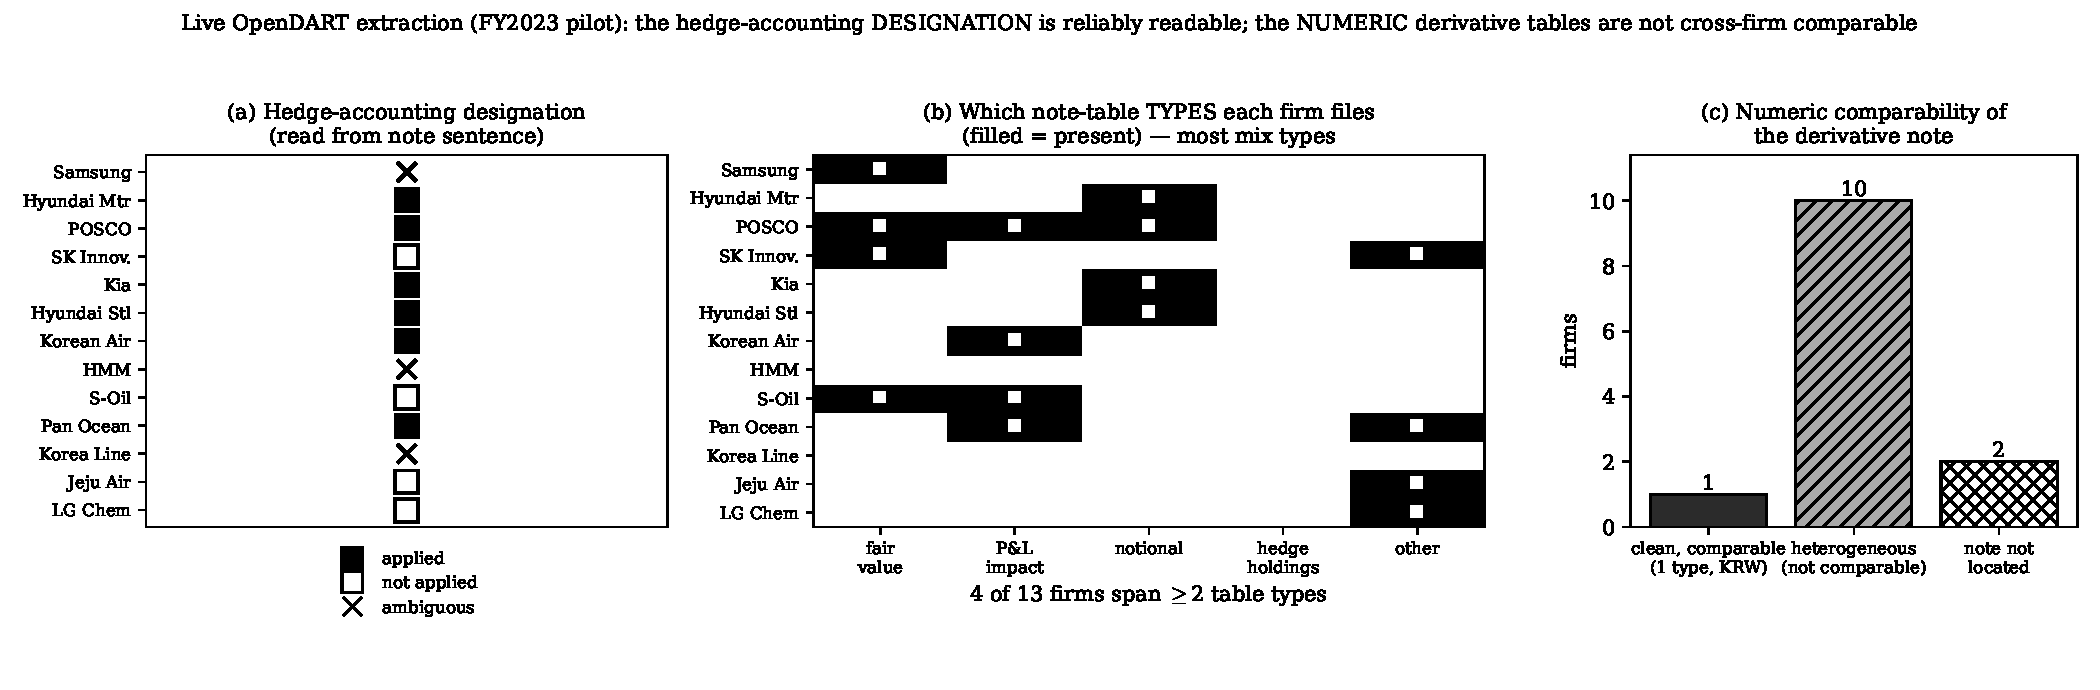
\includegraphics[width=\textwidth]{figures/fig_real_data.pdf}
\caption{Live OpenDART extraction (FY2023 pilot), in black and white. (a) Hedge-accounting designation read from each firm's note sentence: applied (filled), not applied (open), ambiguous ($\times$) -- the one robustly extractable outcome. (b) Which note-table \emph{types} each firm files (filled cell = present); most firms span two or more, so a single parser cannot align them. (c) Numeric comparability of the derivative note: only one of thirteen located notes is a clean single-type table.}
\label{fig:realdata}
\end{figure}

\subsection{Treatment and sample}
\label{sec:sample}

The sample is non-financial KOSPI and KOSDAQ firms over a window spanning several years either side of the first mandatory phase-in. Financial firms are excluded (their derivative use is dealing, not hedging). \emph{Treated}$_i=1$ if firm $i$ falls in a phase whose obligation has commenced; \emph{Post}$_t$ is defined relative to each phase's effective date, so treatment is staggered by $g_i$. Not-yet-covered firms in later phases are the clean control group.

The FX-hedging and hedge-accounting outcomes (H1 FX leg, H2) run on the full non-financial panel. The \emph{commodity}-hedging outcome, however, runs on a restricted subsample, for a measurement reason. \emph{CommodityHedgeRatio} needs a denominator that reflects genuine physical commodity exposure, and cost of goods sold is a poor universal proxy for it: for a refiner or an airline, COGS \emph{is} essentially the priced commodity (crude, jet fuel), but for a chemical, steel, or auto producer, COGS blends raw materials, labor, depreciation, and semi-finished inputs, so a firm can carry large COGS with little tradable-commodity price exposure -- and any commodity-hedge ratio built on it is contaminated. Rather than apply an unreliable proxy panel-wide, the commodity tests are confined to industries whose dominant input is an exchange-traded commodity with an identifiable physical purchase volume -- \emph{oil refining, airlines, shipping, and steel} -- where the derivative-footnote notional can be scaled by a disclosed physical or clearly commodity-dominated purchase figure rather than by blended COGS. This trades sample size for construct validity, the scope chosen for the commodity channel; the FX channel, whose denominator (foreign sales) is clean across industries, carries the broad-panel evidence.

\subsection{Variable definitions}
\label{sec:variables}

\begin{table}[h]
\centering
\small
\begin{tabular}{p{3.2cm} p{6.6cm} p{2.6cm}}
\toprule
Variable & Definition & Units / type \\
\midrule
\emph{HedgeIntensity} & Total derivative notional $/$ total assets & ratio, winsor.\ 1/99 \\
\emph{FXHedgeRatio} & FX-derivative notional $/$ foreign sales & ratio, winsor. \\
\emph{CommodityHedgeRatio} & Commodity-derivative notional $/$ physical (or commodity-dominated) purchases; commodity-exposed subsample only (refining, airlines, shipping, steel) & ratio, winsor. \\
\emph{ClimateHedgeRatio} $h_c$ & Notional of climate-linked instruments (K-ETS emission-allowance derivatives, green/sustainability-linked bond issuance, carbon-price hedges) $/$ carbon exposure (Scope~1$+$2 $\times$ allowance price); disclosing firms only & ratio, sparse \\
\emph{HedgeAccountingDummy} & $1$ if cash-flow-hedge accounting elected (K-IFRS 1109) & binary \\
\emph{RiskEfficiency} & Realized-volatility reduction $/$ hedging cost ($\Delta\mathrm{Vol}/C_H$) & ratio, winsor. \\
\emph{DisclosureIntensity} $d$ & Standardized index of KSSB/ISSB climate-disclosure line items filed & $z$-score \\
\emph{CarbonIntensity} & Scope~1$+$2 emissions $/$ sales (industry-benchmarked) & ratio \\
\emph{DisclosureCost} $a$ & Assurance/audit-fee ratio; reporting-complexity proxy & ratio \\
\emph{DistressCost} $\phi$ & Composite of leverage, Altman-$Z$, credit rating, and \emph{CFvol} (proxy for the latent distress-cost motive; used in H5) & index \\
\emph{Size} & $\ln$(total assets) & ln KRW \\
\emph{Leverage} & Total debt $/$ total assets & ratio, winsor. \\
\emph{MarketToBook} & Market value of equity $/$ book value & ratio, winsor. \\
\emph{ForeignSales} & Foreign sales $/$ total sales & ratio \\
\emph{CFvol} & 12-quarter rolling s.d.\ of operating cash flow $/$ assets & ratio, winsor. \\
\bottomrule
\end{tabular}
\caption{Variable definitions. Continuous variables are winsorized at the 1st/99th percentiles; ratios with denominators near zero (e.g.\ \emph{FXHedgeRatio} for firms with negligible foreign sales) are set missing rather than truncated, and the affected firms enter the FX regressions only. \emph{CommodityHedgeRatio} is defined only on the commodity-exposed subsample (Section~\ref{sec:sample}) to avoid the COGS-as-exposure contamination that afflicts a panel-wide construction. \emph{DisclosureCost} is residualized on size, an internal-control-quality index, and industry before use (Section~\ref{sec:hypotheses}), since the raw proxy is entangled with risk-management capability.}
\label{tab:variables}
\end{table}

\subsection{Mapping the two-risk model to the estimable panel}
\label{sec:mapping}

The model of Section~\ref{sec:model} carries two hedge ratios, $h_f$ (financial) and $h_c$ (climate), and consistency requires being explicit about how each reaches the data -- rather than letting the empirics silently collapse to the financial leg. The financial ratio maps cleanly: $h_f$ is the FX and commodity hedging captured by \emph{FXHedgeRatio}, \emph{CommodityHedgeRatio}, and \emph{HedgeIntensity}, exactly the exposure the companion budget paper (Park, 2026a) prices as a two-factor WTI/USD-KRW position. The climate ratio $h_c$ maps to \emph{ClimateHedgeRatio} -- the notional of climate-linked instruments (K-ETS emission-allowance derivatives, green and sustainability-linked bonds, carbon-price hedges) scaled by carbon exposure -- but this proxy is \emph{sparse}: most Korean non-financial firms did not, over the sample window, hold quantifiable climate-hedging instruments, so $h_c$ is populated only for the disclosing minority (chiefly the carbon-intensive, K-ETS-covered emitters).

This sparsity dictates a two-tier estimation structure. The full-panel tests estimate the financial ratio and the adoption dummy, which is the \emph{financial-risk special case} of the model -- formally the $\phi,\lambda,a$ mechanism operating on the single factor $\sigma_f$, with the climate leg set to zero exposure. The two-risk model is estimated only where it is identified: on the subsample of K-ETS-covered emitters with a non-missing \emph{ClimateHedgeRatio}, where $h_c$, $\sigma_c$, and the cross term $\rho\sigma_f\sigma_c$ are observable and H3's carbon-intensity heterogeneity has bite. The paper thus nests its own reduction: the general two-risk theory is the object, the financial-risk model is its estimable core on the full panel, and the climate leg is an identified extension on the emitter subsample -- and no claim about $h_c$ is made on firms for which it is unmeasured.

\subsection{Winsorization and missing data}
\label{sec:cleaning}

Continuous ratios are winsorized at the 1st and 99th percentiles within each year. Missing derivative-notional fields are treated as structural zeros only when the financial-instruments note affirmatively states no derivative positions; otherwise they are coded missing and multiply imputed for robustness, with results reported both on the imputed and complete-case samples. Firms changing fiscal-year-end or undergoing a merger within the window are flagged and dropped in a robustness cut. The hedge-accounting dummy is validated against the OCI cash-flow-hedge-reserve movement: a non-zero reserve with a zero dummy (or vice versa) is a parsing error and is reconciled by hand.

% =============================================================================
\section{The Executed Study: Korea's Governance-Report Mandate}
\label{sec:executed}

The design of Sections~\ref{sec:design}--\ref{sec:data} was written for the KSSB/ISSB climate-disclosure mandate; that mandate's phase-in has not yet produced a post-period, so it cannot yet be tested. Korea does, however, have two ESG-disclosure mandates with realized adoption: the staggered mandatory corporate-governance report (\emph{gieop-jibaegujo bogoseo}), the G pillar, required of KOSPI issuers with total assets $\ge$ KRW 2 trillion from 2019, $\ge$1tn from 2022, and $\ge$0.5tn from 2024; and the environmental-information disclosure requirement (Environmental Technology and Industry Support Act), which from 2022 obliges listed firms with assets $\ge$ KRW 2 trillion to report quantitative environmental data. This section estimates the effect of both, with the same estimators, outcome parser, and falsification structure the climate test will eventually use. Neither mandate quantifies market-risk exposure -- the dimension the model prices -- so the theory's prediction for both is a null; the section reports whether the data agree.

\subsection{Sample, treatment, and outcomes}
\label{sec:execsample}

From the full OpenDART registry (118{,}482 entities), 2{,}391 KOSPI issuers were screened against \texttt{company.json} (market classification, industry) and their FY2018 consolidated statements, excluding financials (KSIC 64--66). Cohorts were assigned by FY2018 total assets -- an intention-to-treat convention that avoids endogenous threshold-crossing -- into $g{=}2019$ ($\ge$2tn; 100 firms), $g{=}2022$ (1--2tn; 60), $g{=}2024$ (0.5--1tn; 70), and not-yet-treated ($<$0.5tn; 150): 380 firms, with the two upper cohorts close to the population of qualifying KOSPI non-financials. For every firm and fiscal year 2016--2024 the annual report was located, retrieved, and parsed -- 3{,}420 firm-years, 3{,}350 with a filed report -- using the designation parser validated in the pilot of Section~\ref{sec:pilot}. Outcomes: \emph{HedgeAccountingDummy} (1 if the note's operative sentence affirms hedge-accounting designation; 0 if it affirms non-application \emph{or} the filing mentions no derivative instrument, since designation requires an instrument; missing only where derivatives are present but the designation language is ambiguous -- 2{,}609 usable firm-years across 360 firms), \emph{DerivUse} (any derivative-instrument mention; 3{,}350 firm-years), and \emph{ln(1+FXfwd)}, the textual salience of FX-forward disclosure. Treatment $D_{it}=\mathbf 1\{t\ge g_i\}$.

A data-quality note: DART documents filed before 2021 are encoded CP949 rather than UTF-8, and in the initial panel build a decoder default deleted Hangul text from older filings, zeroing all pre-2020 derivative indicators and producing a spurious mandate ``effect'' of $+0.24$. The placebo test below flagged the anomaly (a fake mandate on a not-yet-treated cohort also ``produced'' an effect); correcting the decoder restored economically sensible baselines (a 59\% pre-2019 derivative-usage rate) and the estimates reported here. Both panel versions are archived.

Because treatment is assigned by an asset threshold, there is no covariate overlap between treated and control firms, and regression adjustment on size would extrapolate off the support. Comparability is therefore handled through comparison-set design, and every estimate is reported under three rules: (i) all not-yet-treated firms (the Callaway--Sant'Anna default); (ii) the \emph{adjacent} cohort only -- the next size tier, within roughly a factor of two in assets; and (iii) a \emph{threshold-local} contrast restricted to firms within 50\% of each cutoff on either side. A placebo -- a fake $g{=}2019$ mandate assigned to the 2024 cohort over 2016--2023, when its true obligation had not begun -- estimates residual size-correlated trends directly.

\subsection{Results}
\label{sec:execresults}

Table~\ref{tab:realresults} reports group-time ATTs under all three comparison rules with firm-cluster bootstrap CIs (999 replications), alongside the placebo. Figure~\ref{fig:realevent} shows the event studies with bootstrap bands; Figure~\ref{fig:realrules} displays every estimate against the placebo.

\begin{table}[h]
\centering
\small
\begin{tabular}{lrcccc}
\toprule
Outcome & $N$ & Not-yet & Adjacent cohort & Threshold-local & Placebo \\
\midrule
Hedge-acct.\ designation & 2{,}609 & $-0.005$ & $-0.038$ & $-0.019$ & $+0.060$ \\
 & & {\scriptsize$[-0.068,+0.060]$} & {\scriptsize$[-0.108,+0.033]$} & {\scriptsize$[-0.114,+0.068]$} & {\scriptsize$[-0.052,+0.175]$} \\
Derivative use & 3{,}350 & $-0.050$ & $-0.079$ & $-0.055$ & $+0.047$ \\
 & & {\scriptsize$[-0.113,+0.013]$} & {\scriptsize$[-0.156,-0.015]$} & {\scriptsize$[-0.129,+0.019]$} & {\scriptsize$[-0.048,+0.135]$} \\
ln(1$+$FX-fwd mentions) & 3{,}350 & $+0.092$ & $+0.040$ & $+0.158$ & $+0.102$ \\
 & & {\scriptsize$[-0.037,+0.230]$} & {\scriptsize$[-0.122,+0.170]$} & {\scriptsize$[+0.003,+0.323]$} & {\scriptsize$[-0.107,+0.322]$} \\
\bottomrule
\end{tabular}
\caption{Governance-mandate estimates, OpenDART panel (380 firms, 3{,}420 firm-years, fiscal 2016--2024). Group-time ATTs under three comparison-set rules; 95\% CIs from firm-cluster pairs bootstrap (999 replications). Placebo: fake $g{=}2019$ assigned to the 2024 cohort over 2016--2023 (true effect zero by construction).}
\label{tab:realresults}
\end{table}

Three findings. \emph{First, the real margins are precise nulls, robust to the comparison set.} Hedge-accounting adoption moves $-0.5$pp against a 69\% base rate (CI $[-6.8, +6.0]$pp); derivative usage moves $-5.0$pp against 61\% (CI $[-11.3, +1.3]$pp); and the signs and magnitudes are stable across all three comparison rules -- under the adjacent-cohort rule derivative use is, if anything, significantly \emph{negative} ($-0.079$, CI $[-0.156,-0.015]$). The event-study paths (Figure~\ref{fig:realevent}) are flat through event time. \emph{Second, the placebo is clean at this sample size.} Its point estimates ($+0.05$ to $+0.06$ on the real margins) are statistically indistinguishable from zero, so residual size trends are small relative to the reported CIs, and the nulls are not an artifact of the comparison. \emph{Third, the textual margin does not survive scrutiny.} FX-forward disclosure language rises by an insignificant $+0.092$ log points overall; the one marginally significant reading (threshold-local, $+0.158$) is matched in magnitude by the placebo ($+0.102$), consistent with disclosure verbosity trending with size rather than responding to the mandate -- the reporting-without-real-effects pattern that Christensen, Hail, and Leuz (2021) lead mandatory-CSR research to expect. The carbon-intensity split (H3) yields CIs that include zero in both groups (carbon $-0.034$ $[-0.171,+0.095]$; non-carbon $+0.009$ $[-0.057,+0.071]$) and is reported as inconclusive.

\begin{figure}[h]
\centering
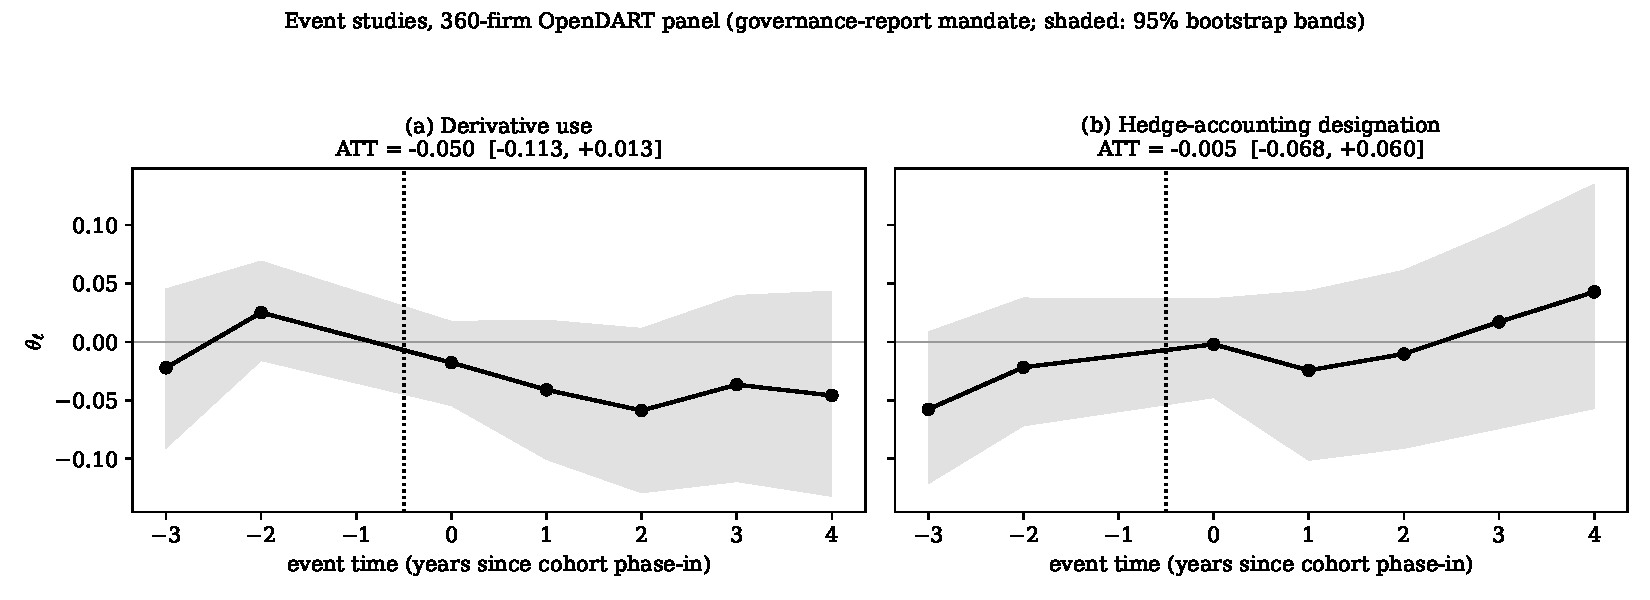
\includegraphics[width=\textwidth]{figures/fig_real_eventstudy.pdf}
\caption{Event studies (380-firm panel; shaded areas are 95\% bootstrap bands): (a) derivative use, (b) hedge-accounting designation. Both paths are flat through the phase-in.}
\label{fig:realevent}
\end{figure}

\begin{figure}[h]
\centering
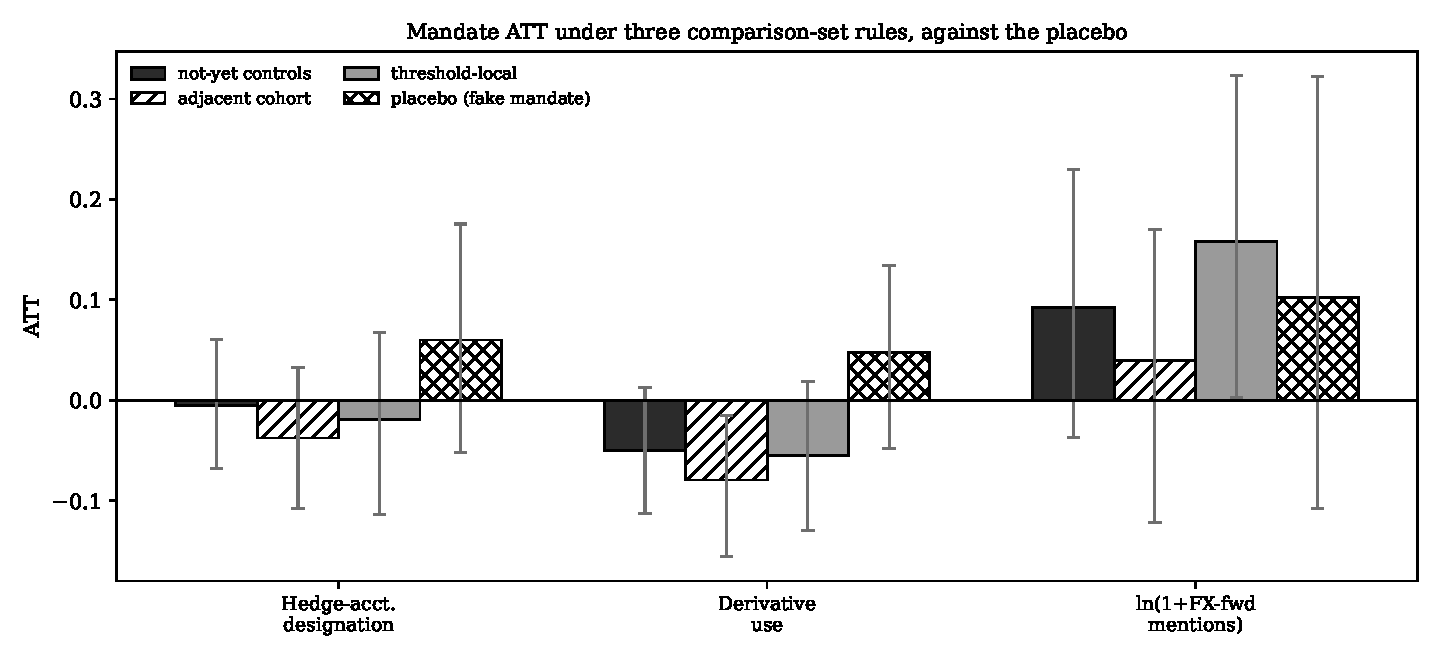
\includegraphics[width=0.9\textwidth]{figures/fig_real_rules.pdf}
\caption{Every governance-mandate ATT under the three comparison-set rules, against the placebo. Real margins cluster at zero across rules; the textual margin's confidence intervals all cross zero and match the placebo's magnitude.}
\label{fig:realrules}
\end{figure}

\subsection{The environmental-information mandate}
\label{sec:epillar}

The second realized mandate provides a sharper test of the same mechanism one rung up the exposure ladder. From 2022, listed firms with assets $\ge$ KRW 2 trillion must disclose quantitative environmental information -- emissions, energy, water, waste -- under the Environmental Technology and Industry Support Act. This E-pillar mandate forces \emph{quantitative} disclosure, but of physical quantities rather than of market-risk exposure; the model therefore still predicts no response in currency and commodity hedging. Estimating the 2022 event on the $\ge$2tn cohort (base year 2021, never-treated controls; the cohort's standing governance obligation is absorbed by the pre-period) gives ATTs of $+0.010$ $[-0.048,+0.063]$ on hedge-accounting designation and $-0.009$ $[-0.069,+0.049]$ on derivative use -- nulls with half-widths near five percentage points -- and $+0.127$ $[-0.038,+0.292]$ on disclosure text. A mandate that compels quantitative environmental reporting moves market-risk hedging no more than the governance report did.

\subsection{What the null means for the theory}
\label{sec:execinterp}

The model gives the nulls a direct interpretation. In Section~\ref{sec:model}, disclosure regulation moves hedging only through $\Lambda(d)=\phi+\lambda e^{-kd}$ -- the price of \emph{residual risk made visible}. The two realized mandates now trace out the bottom of an exposure ladder. A governance report discloses board structure and control without touching exposure at all; a null follows. The environmental-information mandate forces quantitative disclosure, but of physical quantities, not of the market-risk exposure a currency or commodity hedge addresses; a null follows again, and is found, with confidence intervals tight enough to exclude effects beyond roughly six percentage points on either margin. Together the two results say the penalty channel is \emph{risk-specific}: obliging firms to disclose more -- even quantitatively -- does not change hedging unless what must be disclosed is the hedgeable exposure itself. Section~\ref{sec:floor} states this formally: both mandates are binding floors $\underline{d}$ on content orthogonal to $\Lambda$, the cell of the $(\underline{d},\lambda)$ design for which the model's prediction is an exact zero rather than a small effect. That is precisely what the KSSB/ISSB climate standards will require: S2 compels quantification of climate-related \emph{financial} exposure, the top rung of the ladder, and the model predicts H1--H2 should appear there where the lower rungs produced nothing. If the climate mandate's realized post-periods deliver the same null on the same pipeline, the penalty-channel mechanism -- not one mandate's scope -- is rejected. The pipeline, parser, estimators, and placebo architecture run unchanged on that test.

% =============================================================================


% =============================================================================
\section{Robustness and Identification Threats}
\label{sec:robust}

The design's credibility rests on four identification threats, each with a specific answer. I organize the robustness program around them rather than around a list of checks.

\paragraph{Parallel trends.} Identification of $\beta$ requires that treated and control hedging would have moved together absent the mandate. The event study \eqref{eq:eventstudy} tests this on the pre-period leads with a joint Wald test, sup-$t$ uniform bands, and a Rambachan--Roth-style sensitivity of the post-period estimates to bounded pre-trend violations -- so a failure-to-reject on the leads is treated as bounded evidence, not proof. The natural worry that phase order is \emph{endogenous} -- the regulator covers the most-exposed firms first -- threatens levels, not necessarily trends; the event study addresses trends directly, and the not-yet-covered controls are firms the same regulator will treat later, which tightens comparability. The IV/RD around the size-eligibility cutoff (Section~\ref{sec:altid}) exploits that phase membership near the margin is set by the threshold, not by exposure. A pre-phase-in ``treatment'' lead separately tests for pre-emptive hedging; a significant lead is reported under both readings -- rational anticipation (raising the expected penalty) versus a trends violation -- rather than assumed away.

\paragraph{Measurement error.} Three measurement concerns bear on the outcomes. First, derivative notional overstates hedging -- a firm can raise notional without reducing risk (Guay and Kothari, 2003); every test is therefore re-run with fair-value- and sensitivity-based (delta-notional) measures where the footnotes permit, and \emph{RiskEfficiency} (H4) is carried precisely so that a notional rise with flat efficiency is reported as an economically distinct (model-consistent corner) outcome rather than a confirmation. Second, disclosure text is not hedging substance; this is answered by construction, since the outcomes are real balance-sheet and market objects -- derivative notional, OCI cash-flow-hedge-reserve movements, realized volatility -- not disclosure language, and boilerplate would attenuate $\beta$ toward zero, biasing \emph{against} the hypotheses. Third, the commodity denominator (COGS-as-exposure) and the disclosure-cost proxy (capability entanglement) are handled at the construction stage -- the former by the commodity-exposed subsample, the latter by residualization and instrumentation (Sections~\ref{sec:sample},~\ref{sec:hypotheses}).

\paragraph{Staggered-adoption bias.} Because timing varies by tier, two-way fixed effects \eqref{eq:did} is biased by forbidden comparisons of later- to already-treated units (Goodman-Bacon, 2021). The primary estimates are therefore the Callaway--Sant'Anna (2021) group-time ATT against not-yet-covered controls, corroborated by Sun--Abraham (2021) and de Chaisemartin--D'Haultf\oe uille (2020); TWFE is reported only as a benchmark, and a large TWFE-vs-robust gap is itself read as a heterogeneity diagnostic. Alternative treatment coding (obligation date vs.\ first affected fiscal year vs.\ first ISSB-aligned filing) probes sensitivity to the timing definition.

\paragraph{Functional-form dependence.} The penalty $\lambda R e^{-kd}$ is a reduced form. The comparative-statics signs of Section~\ref{sec:compstat} depend only on $\partial P/\partial d<0$ and $\partial P/\partial R>0$, not on the exponential kernel: replacing $e^{-kd}$ with any smooth decreasing attenuation (e.g.\ the power law $(1+kd)^{-1}$) preserves every sign, as noted at \eqref{eq:penalty}. A structural-estimation extension that recovers $(\lambda,k,a,\phi)$ from the data would make the functional form itself testable.

\paragraph{Composition and inference.} Entry, exit, and survivorship are addressed with a balanced-panel cut and inverse-probability weighting; overlapping regulations (contemporaneous tax or K-IFRS amendments) are absorbed by year fixed effects and, where firm-specific, by the triple-difference. All headline results carry firm-clustered, industry$\times$year two-way-clustered, and wild-cluster-bootstrap standard errors -- the last for the small number of treated clusters in the first phase (Bertrand, Duflo, and Mullainathan, 2004).

% =============================================================================
\section{Discussion}
\label{sec:discussion}

Three points deserve emphasis. \emph{First, the mechanism is a price, not a preference.} Disclosure changes hedging in this model only by changing $\Lambda(d)$, the price the firm puts on residual risk; it does not enter the hedging first-order conditions directly. This is what makes the prediction sharp and separable from a general ``responsible firms do more'' story: the disclosure-cost substitution result H(sub) has a sign that only the penalty-channel mechanism produces. \emph{Second, disclosure and hedging are substitutes, not complements, in risk-bearing but complements in observed adoption.} Equation~\eqref{eq:focd} makes them substitutes in the penalty channel (more hedging lowers the disclosure incentive), yet a rise in stringency $\lambda$ raises \emph{both} in equilibrium (H1 and H2 co-move). A researcher who observes disclosure and hedging rising together and infers complementarity would be conflating the response to $\lambda$ with the structural relationship at fixed $\lambda$ -- a distinction the triple-difference on disclosure cost is designed to recover. \emph{Third, the design connects to the rest of the program at the level of the risk price.} The budget paper (Park, 2026a) takes $p_f,p_c$ and the covariance matrix and solves for hedge ratios at a \emph{fixed} risk tolerance; this paper endogenizes that tolerance to the disclosure regime. The hedge-accounting paper (Park, 2026b) shows that the designation architecture -- combined versus split -- changes measured ineffectiveness; here that same election is a firm response margin (H2) to the mandate. And the dynamic-hedging paper (Park, 2026c) prices the cost of running the hedge, which is the $C_H$ that the risk-efficiency outcome (H4) normalizes by. The four papers share one economic object -- a firm pricing and covering joint commodity/currency/climate risk -- viewed at four decision layers.

% =============================================================================
\paragraph{Extensions.}

The design supports four extensions of publishable weight. \emph{(1) The disclosure-quality margin.} Replace the scalar $d$ with a quality-versus-quantity pair and test whether assured/audited disclosure moves hedging more than volume -- separating the penalty channel from a cheap-talk channel. \emph{(2) The cost-of-capital transmission.} Add a mediation layer estimating how much of the hedging response flows through a measured change in cost of debt or equity, linking to Krueger et al.\ (2020) and Bolton--Kacperczyk (2021). \emph{(3) Real effects beyond derivatives.} Extend the outcome set to operational hedging (input sourcing, currency of debt issuance), testing whether financial and operational hedging are substitutes in the disclosure response. \emph{(4) Structural estimation.} With the closed-form equilibrium of Section~\ref{sec:model}, the penalty and disclosure-cost parameters $(\lambda,k,a,\phi)$ are estimable by matching moments of the hedging and disclosure distributions pre/post mandate -- turning the reduced-form DiD into a structural test with counterfactual policy content (e.g.\ the hedging effect of a stricter future phase).

% =============================================================================
\paragraph{Limitations.}

The executed evidence (Section~\ref{sec:executed}) is bounded in scope in three respects. The realized treatments are the governance and environmental-information mandates, not the climate mandate the theory most directly targets, so the nulls constrain the penalty channel's risk-specificity rather than testing its climate form. The outcomes are extensive-margin dummies plus a textual-salience measure, not the continuous hedge ratios of Table~\ref{tab:variables}, whose extraction the pilot showed requires firm-level adjudication; effects on hedging \emph{intensity} within the always-hedging majority are therefore outside what these estimates bound. And treatment is assigned by an asset threshold with no covariate overlap, so identification rests on comparison-set design rather than covariate adjustment -- the three comparison rules and the placebo (which is indistinguishable from zero at this sample size) are the response, but a residual size-trend component within the reported CIs cannot be excluded. The encoding artifact documented in Section~\ref{sec:execsample} separately illustrates the sensitivity of text-based outcome construction to ingestion defaults. The theory collapses the multi-factor commodity/currency exposure of the companion papers into a single financial factor $\sigma_f$ to keep the equilibrium closed-form -- the two-factor structure of Park (2026a) extends the model at the cost of a $3\times3$ system -- and the penalty $\lambda R e^{-kd}$, while given a screening foundation in Section~\ref{sec:problem} that pins the exponential to a verification hazard, remains observationally equivalent to a cost-of-capital repricing channel the model does not separate. Two further gaps between the two-risk theory and the estimable panel are handled explicitly. First, the climate hedge ratio $h_c$ is empirically sparse: outside the K-ETS-covered emitters most firms disclose no quantifiable climate-hedging instrument, so the full-panel tests estimate the financial-risk special case and the two-risk model is identified only on the emitter subsample (Section~\ref{sec:mapping}) -- the reduction is nested and stated, not silent. Second, the disclosure-response boundary \eqref{eq:ddboundary} turns on the latent distress-cost parameter $\phi$, which would render the sign of $\partial d^\star/\partial\lambda$ unfalsifiable if $\phi$ were left unobserved; H5 (Section~\ref{sec:hypotheses}) restores falsifiability by proxying $\phi$ with observable distress-cost measures and testing the implied cross-sectional \emph{ordering} of the disclosure response, but the rescue is only as good as those proxies, and a reader should treat the disclosure-response prediction as the design's most fragile. The identifying variation is a single country's phased mandates, so external validity beyond ISSB-aligned regimes is untested; derivative-notional measurement is coarse and hedge-accounting election is observed only when disclosed. The triple-difference and placebo-timing tests of Section~\ref{sec:design} are constructed specifically to separate the mandate's effect on hedging from a coincident shift in hedging demand driven by the same climate developments that motivated the mandate.

Executing this design on real filings is principally a data-construction task rather than a theoretical or econometric one, and the executed pilot of Section~\ref{sec:pilot} now locates that task precisely  The closed-form solver, the comparative-statics signs, and the staggered-DiD estimator are all machine-verified against model-generated panels (Section~\ref{sec:numerics}); the identification strategy is specified to the coefficient; and the structured front of the pipeline was run live against OpenDART, returning clean financial fields for a real fourteen-firm, four-year sample. Parsing the derivative notes for those firms, however, surfaces a structural obstacle that is not a matter of parser effort: the hedge-accounting \emph{designation} is reliably readable from the note's operative sentence (resolved for ten of fourteen pilot firms, and validated by hand for S-Oil), but the \emph{numeric} derivative tables are filed in incompatible types and units across issuers -- fair-value, notional, and profit-and-loss-impact tables, in KRW and USD, sometimes several within one firm -- so that only one of thirteen located notes is directly comparable (Section~\ref{sec:pilot}). The implication for the empirical program is concrete: the hedge-accounting-adoption outcome (H2) is extractable at scale, but the continuous hedging-intensity outcomes (H1, H4) require firm-level table adjudication or a supervised extraction model rather than a uniform parse, and a full execution should budget for that explicitly. That the binding constraint is disclosure heterogeneity and construct validity -- not the economics or the econometrics -- is where execution of the full design succeeds or fails.

% =============================================================================
\section{Conclusion}
\label{sec:conclusion}

Whether mandatory ESG disclosure changes corporate hedging is, at bottom, a question about the price a firm puts on the risk it chooses not to hedge. This paper makes that intuition precise and then takes it to data. In the model, disclosure enters only through the effective residual-risk price $\Lambda(d)=\phi+\lambda e^{-kd}$; the interior optimum in the two hedge ratios is the closed-form minimum-variance vector $\mathbf 1-\tfrac{1}{2\Lambda(d^\star)}\Sigma^{-1}\mathbf p$; hedging rises unconditionally with stringency while the disclosure response carries the sign of $\phi-\lambda e^{-kd^\star}$; and costlier disclosure raises hedging through substitution ($\partial h_f/\partial a>0$). The executed test runs the paper's staggered, heterogeneity-robust design on Korea's two ESG-disclosure mandates with realized adoption -- the governance report (2019/2022/2024 by asset tier) and the environmental-information requirement (2022, assets $\ge$2tn) -- on a 380-firm, 3{,}420 firm-year panel built from OpenDART filings. The answer is a disciplined null, twice: hedge-accounting adoption at $-0.005$ $[-0.068,+0.060]$ and derivative use at $-0.050$ $[-0.113,+0.013]$ under the governance mandate, $+0.010$ $[-0.048,+0.063]$ and $-0.009$ $[-0.069,+0.049]$ under the environmental mandate, stable across three comparison-set rules, with flat event studies, placebos indistinguishable from zero, and no robust movement even in disclosure text. The nulls are the theory's own reading made empirical: neither mandate forces market-risk exposure into the open, so neither moves the hedging-relevant $\Lambda$ -- the penalty channel is risk-specific -- and the KSSB climate mandate, which compels quantification of the exposure itself, stands as this paper's falsifiable forward test, runnable unchanged on the same pipeline the moment its post-periods exist. Placed alongside its three companions -- static allocation, dynamic hedging, and hedge accounting of the same underlying position -- the paper supplies the missing first link, now with evidence: what makes the firm want to hedge is not disclosure obligation per se, but disclosure that prices the risk it would otherwise carry quietly.

% =============================================================================
\appendix
\section{Comparative Statics via the Implicit Function Theorem}
\label{sec:appendix}

The general-equilibrium signs of Section~\ref{sec:compstat} follow from totally differentiating the equilibrium system $\{$\eqref{eq:linsys}, \eqref{eq:focd}$\}$. Stack the equilibrium conditions as $F(\mathbf u,d;\theta)=0$ for parameter $\theta$:
\begin{equation}
F_1: 2\Lambda(d)\Sigma\mathbf u-\mathbf p=0,\qquad F_2: 2ad-k\lambda e^{-kd}\,\mathbf u^\top\Sigma\mathbf u=0.
\end{equation}
The Jacobian with respect to $(\mathbf u,d)$ is
\begin{equation}
J=\begin{pmatrix} 2\Lambda\Sigma & 2\Lambda'(d)\Sigma\mathbf u\\[2pt] -2k\lambda e^{-kd}(\Sigma\mathbf u)^\top & 2a+k^2\lambda e^{-kd}\,\mathbf u^\top\Sigma\mathbf u\end{pmatrix},
\end{equation}
whose determinant is positive under the second-order condition \eqref{eq:soc} (it is the same Schur complement, up to the positive factor $\det(2\Lambda\Sigma)$). For $\theta=\lambda$,
\begin{equation}
-\frac{\partial F}{\partial\lambda}=\begin{pmatrix} -2e^{-kd}\Sigma\mathbf u\\ k e^{-kd}\mathbf u^\top\Sigma\mathbf u\end{pmatrix},
\end{equation}
and Cramer's rule on $J\,(\partial\mathbf u/\partial\lambda,\partial d/\partial\lambda)^\top=-\partial F/\partial\lambda$ delivers $\partial\mathbf u^\star/\partial\lambda<0$ componentwise (the unhedged fraction falls), hence $\partial h_f^\star/\partial\lambda>0$, confirming H1 inclusive of the disclosure feedback. The disclosure derivative is not unconditionally signed. Working the scalar fixed point \eqref{eq:dfixed} directly -- take logs, $\ln(8a)+\ln d+2\ln\Lambda=\ln(k\lambda\kappa)-kd$, and differentiate totally in $\lambda$ -- collects to
\begin{equation}
\frac{\partial d^\star}{\partial\lambda}\Big[\tfrac{1}{d^\star}+k-\tfrac{2k\lambda e^{-kd^\star}}{\Lambda}\Big]=\frac{1}{\lambda}-\frac{2e^{-kd^\star}}{\Lambda}.
\end{equation}
The bracket on the left is positive at an interior optimum, so the sign of $\partial d^\star/\partial\lambda$ is the sign of the right-hand side, $\tfrac{1}{\lambda}-\tfrac{2e^{-kd^\star}}{\Lambda}$, which is positive iff $\Lambda>2\lambda e^{-kd^\star}$, i.e.\ iff $\phi>\lambda e^{-kd^\star}$ -- exactly the boundary \eqref{eq:ddboundary}. The same construction with $\theta=a$ gives $\partial d^\star/\partial a<0$ and $\partial\mathbf u^\star/\partial a<0$, hence $\partial h_f^\star/\partial a>0$, establishing the structural (level) form of H(sub).

% =============================================================================
\section{Second-Order Conditions, Existence, and Uniqueness}
\label{sec:soc}

The Hessian of $\Pi$ blocks as
\begin{equation}
H=\begin{pmatrix} 2\Lambda\,\Sigma & \Lambda'(d)\,\nabla_{h}R\\[2pt] \Lambda'(d)\,\nabla_{h}R^\top & 2a+\Lambda''(d)R\end{pmatrix},
\qquad \nabla_h R=-2\Sigma\mathbf u,\ \ \Lambda''(d)=k^2\lambda e^{-kd}>0.
\end{equation}
The hedge block $2\Lambda\Sigma$ is positive definite (Section~\ref{sec:hedgesol}). The disclosure diagonal $2a+\Lambda''R=2a+k^2\lambda e^{-kd}R>0$. By the Schur-complement criterion, $H\succ 0$ -- so the interior critical point is the unique global minimum -- iff
\begin{equation}
2a+k^2\lambda e^{-kd}R \;>\; \Lambda'(d)^2\,\nabla_h R^\top(2\Lambda\Sigma)^{-1}\nabla_h R
= \frac{k^2\lambda^2 e^{-2kd}}{2\Lambda}\cdot 2\,\mathbf u^\top\Sigma\mathbf u=\frac{k^2\lambda^2 e^{-2kd}R}{\Lambda},
\label{eq:soc}
\end{equation}
using $\nabla_h R^\top\Sigma^{-1}\nabla_h R=4\mathbf u^\top\Sigma\mathbf u=4R$. Condition~\eqref{eq:soc} rearranges to a lower bound on the disclosure-cost curvature,
\begin{equation}
a\;>\;\frac{k^2\lambda\,e^{-kd}R}{2}\left(\frac{\lambda e^{-kd}}{\Lambda}-1\right)=-\frac{k^2\lambda e^{-kd}R}{2}\cdot\frac{\phi}{\Lambda}\;\le 0,
\end{equation}
which is \emph{automatically satisfied} whenever $\phi\ge0$ and $a>0$: the right-hand side is non-positive, so any positive disclosure-cost curvature guarantees a strict global minimum. The equilibrium of Sections~\ref{sec:hedgesol}--\ref{sec:dsol} is thus unique and well-defined under the model's maintained sign restrictions, with no further parameter conditions needed -- the substitutability between disclosure and hedging (the negative cross term) is exactly what makes the joint problem convex here.


\section{Numerical Validation of the Model and the Estimators}
\label{sec:numerics}

Before any real filing is parsed, two things can and should be checked: that the equilibrium of Section~\ref{sec:model} is what the closed form claims, and that the estimators of Section~\ref{sec:design} recover the predicted signs when the data are generated by the model itself. A companion engine does both. Its scope is internal -- it validates the design's logic on model-generated data and is \emph{not} evidence about real firms -- but it is the same discipline the companion trilogy applies to its pricing and accounting engines: certify the machinery on cases with a known answer before trusting it on cases without one.

\subsection{Structural solver and comparative-statics verification}
\label{sec:solververif}

The firm's program \eqref{eq:objective} is solved two independent ways -- the closed-form fixed point of Sections~\ref{sec:hedgesol}--\ref{sec:dsol} and a direct multi-start box-constrained minimization of $\Pi$ -- and the two are required to agree. At the baseline calibration ($\sigma_f{=}0.30$, $\sigma_c{=}0.15$, $\rho{=}0.20$, $p_f{=}0.030$, $p_c{=}0.020$, $\phi{=}0.15$, $\lambda{=}0.60$, $k{=}1.0$, $a{=}0.05$) they agree to $8.8\times10^{-9}$, giving $h_f^\star=0.8213$, $h_c^\star=0.4476$, $d^\star=0.0648$, $R^\star=1.15\times10^{-2}$. Every comparative-statics sign of Table~\ref{tab:compstat} is then verified by re-solving the full equilibrium under parameter shocks (Table~\ref{tab:signverif}). The delicate one is the disclosure response: the measured $\partial d^\star/\partial\lambda=-0.065$ is \emph{negative} here, and it should be -- at this calibration $\phi-\lambda e^{-kd^\star}=-0.412<0$, so the boundary \eqref{eq:ddboundary} predicts exactly the negative sign the solver returns. The substitution channel $\partial h_f^\star/\partial a=+0.190>0$ (with $\partial d^\star/\partial a=-1.346<0$) is confirmed as a genuine but modest level effect. Figure~\ref{fig:modelverif} shows the certified curves.

\begin{table}[h]
\centering
\small
\begin{tabular}{llrl}
\toprule
Derivative & Predicted & Measured & Verdict \\
\midrule
$\partial h_f^\star/\partial\lambda$ & $+$ & $+0.244$ & pass \\
$\partial d^\star/\partial\lambda$ & $\operatorname{sign}(\phi-\lambda e^{-kd^\star})$ & $-0.065$ \ ($\phi-\lambda e^{-kd^\star}=-0.412$) & pass (boundary) \\
$\partial h_f^\star/\partial a$ (H(sub)) & $+$ & $+0.190$ & pass \\
$\partial d^\star/\partial a$ & $-$ & $-1.346$ & pass \\
$\partial h_f^\star/\partial p_f$ & $-$ & $<0$ & pass \\
$\partial h_f^\star/\partial\sigma_f$ & $+$ & $>0$ & pass \\
$\partial h_f^\star/\partial\rho$ & sign of \eqref{eq:dhdrho} & matches & pass \\
\bottomrule
\end{tabular}
\caption{Comparative-statics verification. Signs obtained by re-solving the full equilibrium (closed form, including the $d^\star$ feedback) under $\pm$ shocks, checked against the analytic predictions of Section~\ref{sec:compstat}. The disclosure/stringency derivative is checked against the derived boundary \eqref{eq:ddboundary}, not against a fixed sign.}
\label{tab:signverif}
\end{table}

\begin{figure}[h]
\centering
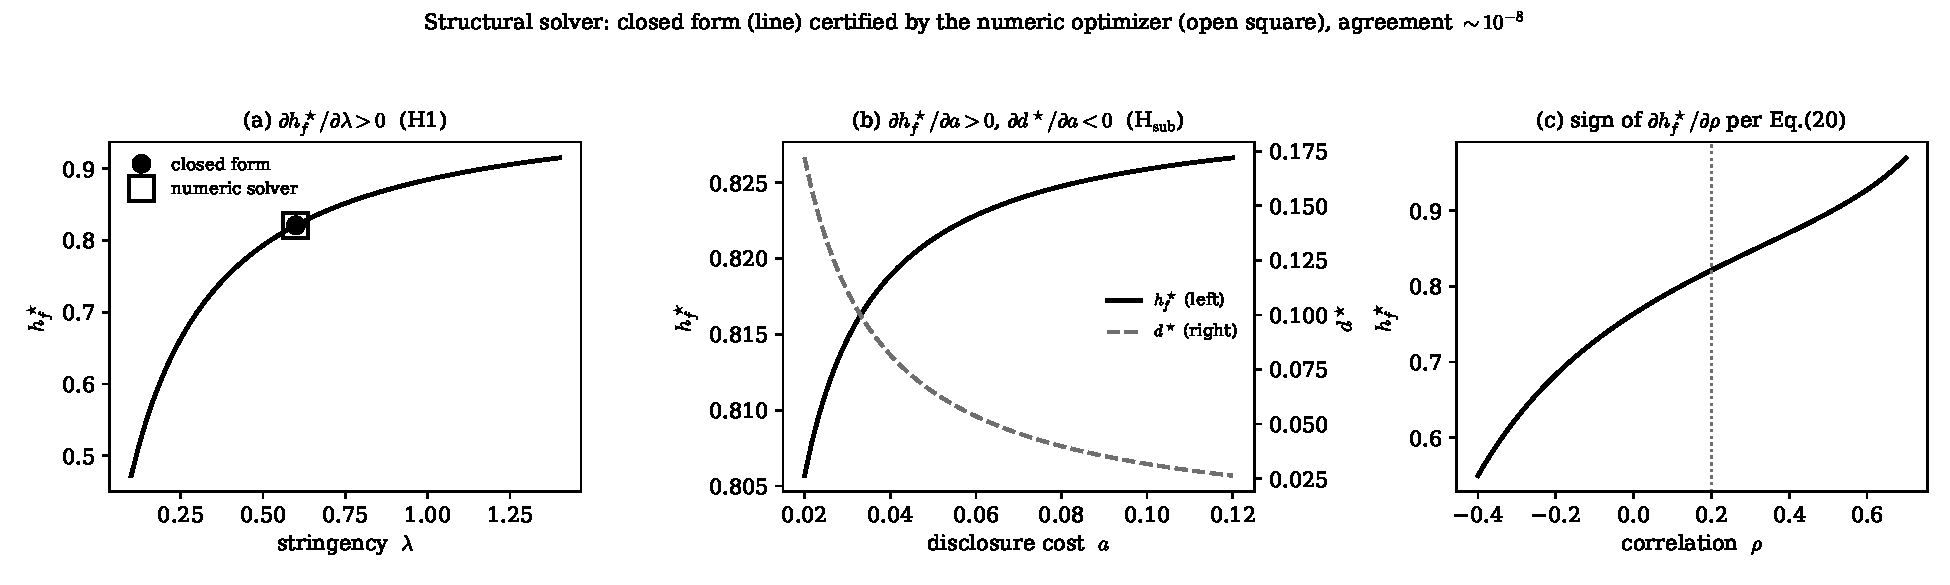
\includegraphics[width=\textwidth]{figures/fig_model_verification.pdf}
\caption{Structural solver. Closed-form equilibrium (line) certified by the independent numeric optimizer ($\times$, panel a). (a) $h_f^\star$ rising in stringency $\lambda$ (H1). (b) $h_f^\star$ rising and $d^\star$ falling in disclosure cost $a$ -- the substitution channel H(sub). (c) $h_f^\star$ rising in correlation $\rho$ over the calibrated range, the sign given by Eq.~\eqref{eq:dhdrho}.}
\label{fig:modelverif}
\end{figure}

\subsection{Recovery on model-generated staggered panels}
\label{sec:didmc}

A synthetic panel ($N{=}900$ firms, $T{=}10$ periods, cohorts phasing in at $g\in\{4,6,\infty\}$) is generated from the structural DGP: the mandate raises $\lambda$ for treated firms, with a larger jump for carbon-intensive firms (the H3 channel), and the hedging response phases in over three years, so treatment effects are dynamic and -- with staggered timing -- two-way fixed effects is expected to be biased. Table~\ref{tab:didrecovery} reports the result. The Callaway--Sant'Anna group-time ATT recovers the true average effect almost exactly ($0.0622$ vs.\ $0.0621$), while TWFE understates it by $12\%$ ($0.0549$), the textbook heterogeneity-with-dynamics bias; pre-trend coefficients are two orders of magnitude below the effect ($\max|\theta_{\ell<0}|=2.9\times10^{-4}$ vs.\ ATT $6.2\times10^{-2}$). Hedge-accounting adoption (H2, anchored to the hedging level) and the carbon-intensity heterogeneity (H3) both come through with the predicted signs. Figure~\ref{fig:didrecovery} shows the event-study path -- flat before, ramping after -- and the estimator comparison.

\begin{table}[h]
\centering
\small
\begin{tabular}{lrl}
\toprule
Quantity & Value & Note \\
\midrule
True ATT (model)                 & $0.0621$ & average realized effect on $h_f$ \\
Callaway--Sant'Anna ATT          & $0.0622$ & error $+5\times10^{-5}$ \\
TWFE ATT                         & $0.0549$ & error $-7.2\times10^{-3}$ (biased) \\
$\max|\theta_\ell|$, $\ell<-1$   & $0.00029$ & pre-trend (parallel-trends check) \\
H2: adoption DiD coefficient     & $0.706$ & positive (hedging-level channel) \\
H3: ATT carbon vs non-carbon     & $0.0717$ vs $0.0518$ & stronger where climate risk larger \\
\bottomrule
\end{tabular}
\caption{Estimator recovery on model-generated staggered panels. The heterogeneity-robust group-time ATT recovers the true effect; two-way fixed effects is biased downward under dynamic effects and staggered timing, motivating the estimator choice of Section~\ref{sec:staggered}.}
\label{tab:didrecovery}
\end{table}

\begin{figure}[h]
\centering
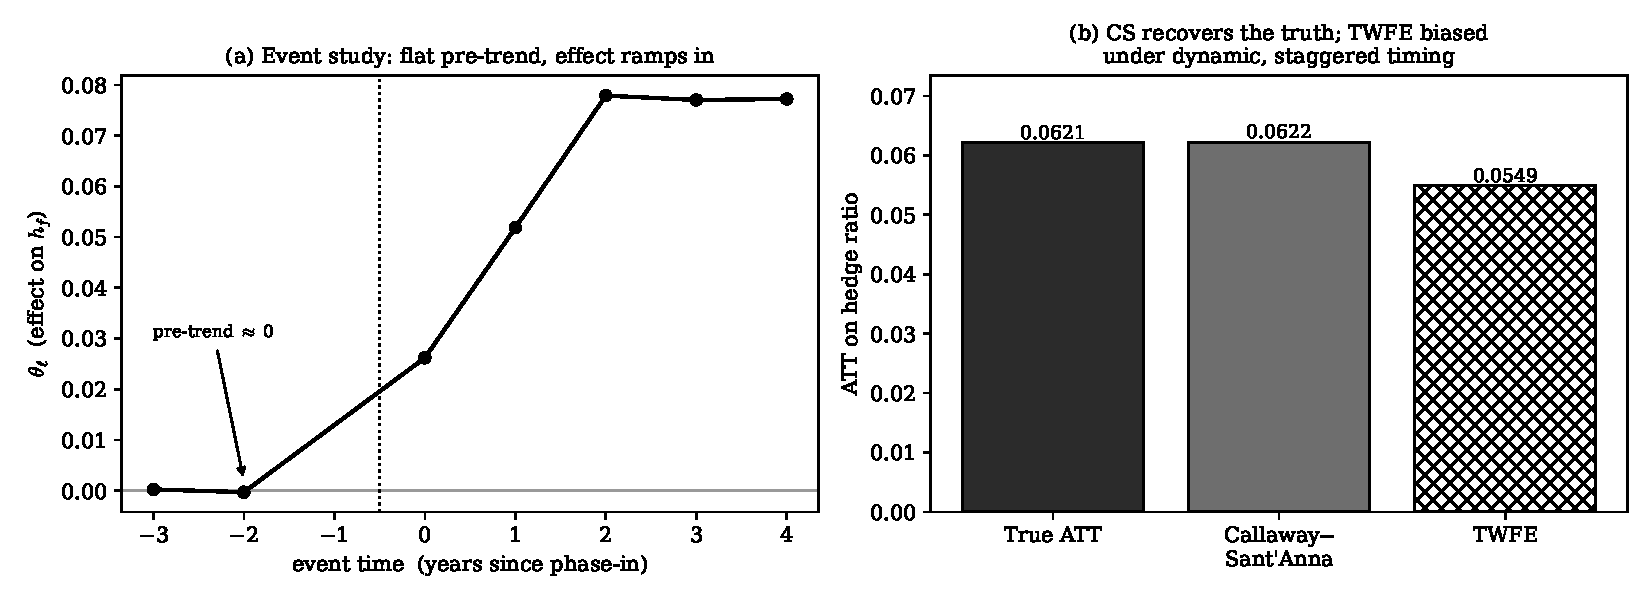
\includegraphics[width=0.95\textwidth]{figures/fig_did_recovery.pdf}
\caption{Design recovery. (a) Event study on model-generated data: flat pre-trend, effect ramping in over three post-treatment years. (b) The Callaway--Sant'Anna ATT recovers the true model ATT; TWFE understates it under heterogeneous, dynamic timing.}
\label{fig:didrecovery}
\end{figure}

\subsection{H(sub) is exactly the fragile prediction}
\label{sec:hsubverif}

The engine tests the identification worry of Section~\ref{sec:hypotheses} directly. On a cross-section of treated firms whose disclosure cost $a$ is \emph{exogenous}, the slope of hedging on $a$ is $+0.139$ -- the structural $\partial h_f^\star/\partial a>0$ made visible. Introducing a capability confound of plausible size -- letting the same latent (lack of) sophistication that raises disclosure cost also depress risk-management capability -- drives the naive slope to $-1.708$, flipping its sign entirely; controlling for the capability index restores it to $+0.170$ (Figure~\ref{fig:hsub}). This is H(sub)'s fragility made quantitative: the substitution effect is real but second-order, so it is precisely the prediction a realistic confound can overturn, and only a design that purges the capability content of the disclosure-cost proxy (Section~\ref{sec:hypotheses}) can identify it. The engine thus validates both the confirmatory predictions and the boundary condition under which the exploratory one holds.

\begin{figure}[h]
\centering
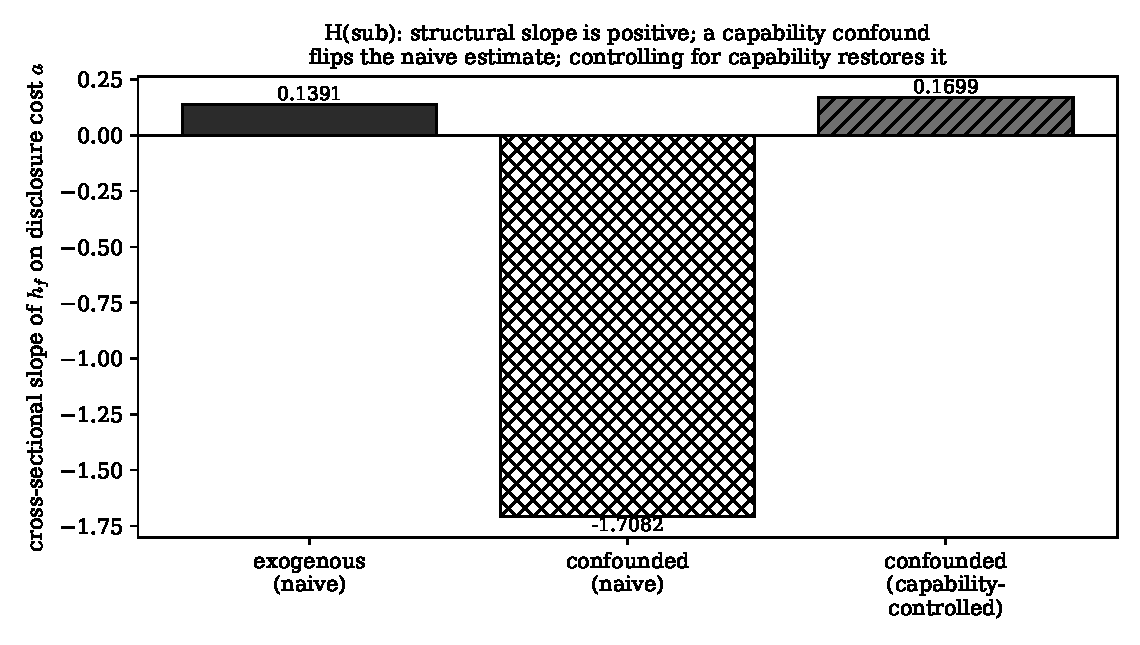
\includegraphics[width=0.72\textwidth]{figures/fig_hsub.pdf}
\caption{H(sub) fragility. Cross-sectional slope of treated-firm hedging on disclosure cost $a$: positive when $a$ is exogenous (structural $\partial h_f^\star/\partial a>0$), flipped negative by a capability confound, restored positive by controlling for capability. The substitution channel is real but second-order, hence identifiable only with the safeguards of Section~\ref{sec:hypotheses}.}
\label{fig:hsub}
\end{figure}

% =============================================================================
\begin{thebibliography}{99}

\bibitem{abadie2010} Abadie, A., A. Diamond, and J. Hainmueller (2010). ``Synthetic Control Methods for Comparative Case Studies.'' \emph{Journal of the American Statistical Association} 105(490), 493--505.

\bibitem{adler1984} Adler, M., and B. Dumas (1984). ``Exposure to Currency Risk: Definition and Measurement.'' \emph{Financial Management} 13(2), 41--50.

\bibitem{allayannis2001} Allayannis, G., and J. P. Weston (2001). ``The Use of Foreign Currency Derivatives and Firm Market Value.'' \emph{Review of Financial Studies} 14(1), 243--276.

\bibitem{anderson1981} Anderson, R. W., and J.-P. Danthine (1981). ``Cross Hedging.'' \emph{Journal of Political Economy} 89(6), 1182--1196.

\bibitem{bartram2011} Bartram, S. M., G. W. Brown, and J. Conrad (2011). ``The Effects of Derivatives on Firm Risk and Value.'' \emph{Journal of Financial and Quantitative Analysis} 46(4), 967--999.

\bibitem{bertrand2004} Bertrand, M., E. Duflo, and S. Mullainathan (2004). ``How Much Should We Trust Differences-in-Differences Estimates?'' \emph{Quarterly Journal of Economics} 119(1), 249--275.

\bibitem{bolton2021} Bolton, P., and M. Kacperczyk (2021). ``Do Investors Care about Carbon Risk?'' \emph{Journal of Financial Economics} 142(2), 517--549.

\bibitem{callaway2021} Callaway, B., and P. H. C. Sant'Anna (2021). ``Difference-in-Differences with Multiple Time Periods.'' \emph{Journal of Econometrics} 225(2), 200--230.

\bibitem{chaisemartin2020} de Chaisemartin, C., and X. D'Haultf\oe uille (2020). ``Two-Way Fixed Effects Estimators with Heterogeneous Treatment Effects.'' \emph{American Economic Review} 110(9), 2964--2996.

\bibitem{chen2018} Chen, Y.-C., M. Hung, and Y. Wang (2018). ``The Effect of Mandatory CSR Disclosure on Firm Profitability and Social Externalities: Evidence from China.'' \emph{Journal of Accounting and Economics} 65(1), 169--190.

\bibitem{christensen2021} Christensen, H. B., L. Hail, and C. Leuz (2021). ``Mandatory CSR and Sustainability Reporting: Economic Analysis and Literature Review.'' \emph{Review of Accounting Studies} 26(3), 1176--1248.

\bibitem{downar2021} Downar, B., J. Ernstberger, S. Reichelstein, S. Schwenen, and A. Zaklan (2021). ``The Impact of Carbon Disclosure Mandates on Emissions and Financial Operating Performance.'' \emph{Review of Accounting Studies} 26(3), 1137--1175.

\bibitem{dye1986} Dye, R. A. (1986). ``Proprietary and Nonproprietary Disclosures.'' \emph{Journal of Business} 59(2), 331--366.

\bibitem{ederington1979} Ederington, L. H. (1979). ``The Hedging Performance of the New Futures Markets.'' \emph{Journal of Finance} 34(1), 157--170.

\bibitem{engle2020} Engle, R. F., S. Giglio, B. Kelly, H. Lee, and J. Stroebel (2020). ``Hedging Climate Change News.'' \emph{Review of Financial Studies} 33(3), 1184--1216.

\bibitem{froot1993} Froot, K. A., D. S. Scharfstein, and J. C. Stein (1993). ``Risk Management: Coordinating Corporate Investment and Financing Policies.'' \emph{Journal of Finance} 48(5), 1629--1658.

\bibitem{garman1983} Garman, M. B., and S. W. Kohlhagen (1983). ``Foreign Currency Option Values.'' \emph{Journal of International Money and Finance} 2(3), 231--237.

\bibitem{geczy1997} G\'eczy, C., B. A. Minton, and C. Schrand (1997). ``Why Firms Use Currency Derivatives.'' \emph{Journal of Finance} 52(4), 1323--1354.

\bibitem{glaum2011} Glaum, M., and A. Kl\"ocker (2011). ``Hedge Accounting and Its Influence on Financial Hedging: When the Tail Wags the Dog.'' \emph{Accounting and Business Research} 41(5), 459--489.

\bibitem{goodmanbacon2021} Goodman-Bacon, A. (2021). ``Difference-in-Differences with Variation in Treatment Timing.'' \emph{Journal of Econometrics} 225(2), 254--277.

\bibitem{graham2002} Graham, J. R., and D. A. Rogers (2002). ``Do Firms Hedge in Response to Tax Incentives?'' \emph{Journal of Finance} 57(2), 815--839.

\bibitem{grewal2019} Grewal, J., E. J. Riedl, and G. Serafeim (2019). ``Market Reaction to Mandatory Nonfinancial Disclosure.'' \emph{Management Science} 65(7), 3061--3084.

\bibitem{guay2003} Guay, W., and S. P. Kothari (2003). ``How Much Do Firms Hedge with Derivatives?'' \emph{Journal of Financial Economics} 70(3), 423--461.

\bibitem{hong2019} Hong, H., F. W. Li, and J. Xu (2019). ``Climate Risks and Market Efficiency.'' \emph{Journal of Econometrics} 208(1), 265--281.

\bibitem{iasb2014} IASB (2014). \emph{IFRS~9 Financial Instruments}. London: IFRS Foundation.

\bibitem{ilhan2023} Ilhan, E., P. Krueger, Z. Sautner, and L. T. Starks (2023). ``Climate Risk Disclosure and Institutional Investors.'' \emph{Review of Financial Studies} 36(7), 2617--2650.

\bibitem{jinjorion2006} Jin, Y., and P. Jorion (2006). ``Firm Value and Hedging: Evidence from U.S. Oil and Gas Producers.'' \emph{Journal of Finance} 61(2), 893--919.

\bibitem{krueger2020} Krueger, P., Z. Sautner, and L. T. Starks (2020). ``The Importance of Climate Risks for Institutional Investors.'' \emph{Review of Financial Studies} 33(3), 1067--1111.

\bibitem{krueger2024} Krueger, P., Z. Sautner, D. Y. Tang, and R. Zhang (2024). ``The Effects of Mandatory ESG Disclosure around the World.'' \emph{Journal of Accounting Research} 62(5), 1795--1847.

\bibitem{nance1993} Nance, D. R., C. W. Smith, and C. W. Smithson (1993). ``On the Determinants of Corporate Hedging.'' \emph{Journal of Finance} 48(1), 267--284.

\bibitem{panaretou2013} Panaretou, A., M. B. Shackleton, and P. A. Taylor (2013). ``Corporate Risk Management and Hedge Accounting.'' \emph{Contemporary Accounting Research} 30(1), 116--139.

\bibitem{parka2026} Park, J. (2026a). ``Optimal WTI--FX Hedge Ratios Under a Fixed Budget.'' Working paper, Pusan National University.

\bibitem{parkb2026} Park, J. (2026b). ``IFRS~9 Hedge Accounting for a Quanto Knock-Out Structure.'' Working paper, Pusan National University.

\bibitem{parkc2026} Park, J. (2026c). ``Dynamic Delta Hedging of a Quanto Knock-Out Option Under Jump-Diffusion.'' Working paper, Pusan National University.

\bibitem{smith1985} Smith, C. W., and R. M. Stulz (1985). ``The Determinants of Firms' Hedging Policies.'' \emph{Journal of Financial and Quantitative Analysis} 20(4), 391--405.

\bibitem{stulz1996} Stulz, R. M. (1996). ``Rethinking Risk Management.'' \emph{Journal of Applied Corporate Finance} 9(3), 8--25.

\bibitem{sunabraham2021} Sun, L., and S. Abraham (2021). ``Estimating Dynamic Treatment Effects in Event Studies with Heterogeneous Treatment Effects.'' \emph{Journal of Econometrics} 225(2), 175--199.

\bibitem{townsend1979} Townsend, R. M. (1979). ``Optimal Contracts and Competitive Markets with Costly State Verification.'' \emph{Journal of Economic Theory} 21(2), 265--293.

\bibitem{tufano1996} Tufano, P. (1996). ``Who Manages Risk? An Empirical Examination of Risk Management Practices in the Gold Mining Industry.'' \emph{Journal of Finance} 51(4), 1097--1137.

\end{thebibliography}

\end{document}
